\documentclass[12pt]{article}

\usepackage{iftex}
\usepackage[provide=*, brazilian]{babel}
\usepackage{sbc-template}
\ifPDFTeX
  \usepackage[utf8]{inputenc}
  \IfFileExists{ptmr8t.tfm}{}{%
    \renewcommand{\rmdefault}{cmr}%
    \renewcommand{\sfdefault}{cmss}%
    \renewcommand{\ttdefault}{cmtt}%
  }
  \usepackage[T1]{fontenc}
\else
  \usepackage{fontspec}
  \IfFontExistsTF{Nimbus Roman}{\setmainfont{Nimbus Roman}}{}
  \IfFontExistsTF{Nimbus Sans}{\setsansfont{Nimbus Sans}}{}
  \IfFontExistsTF{Nimbus Mono PS}{\setmonofont{Nimbus Mono PS}[Scale=MatchLowercase]}{}
\fi
\usepackage{graphicx}
\usepackage{url}
\usepackage{amsmath,amssymb}
\usepackage{booktabs}
\usepackage{array}
\usepackage{xcolor}
\usepackage{placeins}
\usepackage{hyperref}

\hypersetup{
  colorlinks=true,
  linkcolor=black,
  citecolor=black,
  urlcolor=blue!60!black
}

\sloppy

% Inclusão condicional de figuras e tabelas geradas automaticamente por `python -m src.cli analyze`.
\newcommand{\includeFigIfExists}[4]{%
  \begin{figure}[htbp]
    \centering
    \IfFileExists{#1}{%
      \includegraphics[width=\linewidth]{#1}%
    }{%
      \fcolorbox{red!50!black}{red!4}{%
        \begin{minipage}{0.92\linewidth}
          \centering\small\vspace{0.6em}
          \textbf{Figura ainda não gerada (\texttt{\detokenize{#1}})}\\
          #4
          \vspace{0.6em}
        \end{minipage}%
      }%
    }
    \caption{#2}
    \label{#3}
  \end{figure}
}

\newcommand{\includeTableIfExists}[4]{%
  \begin{table}[htbp]
    \centering
    \caption{#2}
    \label{#3}
    \scriptsize
    \IfFileExists{#1}{%
      \resizebox{\linewidth}{!}{\input{#1}}%
    }{%
      \fcolorbox{red!50!black}{red!4}{%
        \begin{minipage}{0.92\linewidth}
          \centering\small\vspace{0.5em}
          \textbf{Tabela ainda não gerada (\texttt{\detokenize{#1}})}\\
          #4
          \vspace{0.5em}
        \end{minipage}%
      }%
    }
  \end{table}
}

\title{Trabalho Prático 2 - Análise Empírica e Otimização para o Caixeiro Viajante}

\author{Bernardo Zschaber Morato Nogueira\inst{1}, Mateus Matsura Teles Costa\inst{1},\\
  Pedro Rangel Ferreira de Aguiar\inst{1}}

\address{Departamento de Ciência da Computação -- Instituto de Ciências Exatas (ICEx)\\
  Universidade Federal de Minas Gerais (UFMG) -- Belo Horizonte -- MG -- Brasil
  \email{\{bernardozschaber, matsuramateus, pedrorangel\}@dcc.ufmg.br}
}

\begin{document}

\maketitle

\begin{abstract}
This paper presents an algorithmic audit, a gradual optimization study, and a topological
sensitivity analysis for the 2D Euclidean Traveling Salesman Problem (\texttt{EUC\_2D}) across
15 native-coordinate TSPLIB instances ($N \in [10, 70]$). We analyze incremental refactorings
across Twice-Around-The-Tree, Christofides (dense Prim, odd-subgraph Blossom isolation, and
linear Hierholzer), five warm-start strategies (including an $O(N^2 \log N)$ lazy-heap
convex-hull insertion), and four Branch-and-Bound versions (\texttt{v0}--\texttt{v3}: GPU
batching, in-place DFS, $\Theta(1)$ degree-2 bounds, bitmasking, and internal symmetry
breaking), evaluating complexity scaling, pruning trade-offs, and adversarial geometries.
\end{abstract}

\begin{resumo}
Este artigo apresenta uma auditoria algorítmica, um estudo de otimização gradual e uma análise
de sensibilidade topológica para o Problema do Caixeiro Viajante Euclidiano 2D
(\texttt{EUC\_2D}) em 15 instâncias TSPLIB de coordenadas nativas ($N \in [10, 70]$).
Analisamos refatorações incrementais no Twice-Around-The-Tree, em Christofides (Prim denso,
isolamento do subgrafo ímpar e Hierholzer linear), em cinco estratégias de \textit{warm-start}
(incluindo inserção em fecho convexo $O(N^2 \log N)$) e em quatro versões do Branch-and-Bound
(\texttt{v0}--\texttt{v3}: lotes em GPU, DFS \textit{in-place}, limites $\Theta(1)$,
\textit{bitmask} e quebra de simetria), investigando complexidade empírica, poda e geometrias
adversariais.
\end{resumo}

\section{Introdução}
\label{sec:introducao}

O Problema do Caixeiro Viajante (\textit{Traveling Salesman Problem}: TSP) consiste
em determinar, para um grafo completo não direcionado $G = (V, E)$ com $|V| = N$ vértices e
uma função de custo não negativa $c: E \rightarrow \mathbb{R}_{\ge 0}$, um circuito
hamiltoniano $H^*$ de soma de arestas mínima que visite cada vértice exatamente uma vez e
retorne à origem \cite{cormen2009clrs,levitin2012design}. Neste trabalho, concentramos o estudo
no caso geométrico conhecido como TSP Euclidiano bidimensional (\texttt{EUC\_2D}), no qual cada
vértice $v_i \in V$ corresponde a um ponto $p_i = (x_i, y_i) \in \mathbb{R}^2$ e o custo de
cada aresta é dado pela distância euclidiana $c(u, v) = \|p_u - p_v\|_2$. Por satisfazer a
desigualdade triangular, essa família de instâncias admite algoritmos polinomiais com
garantias formais de qualidade, como \textit{Twice-Around-The-Tree} (fator de aproximação $2$) \cite{rosenkrantz1977analysis} e 
o algoritmo de Christofides (fator de $1{,}5$)
\cite{christofides1976worst}, ao passo que a obtenção de soluções comprovadamente ótimas exige
técnicas de enumeração implícita com poda, como \textit{Branch-and-Bound}
\cite{levitin2012design}.

Embora as propriedades teóricas dessas abordagens sejam amplamente estabelecidas na literatura,
a passagem da descrição abstrata em livro-texto para um sistema executável revela uma lacuna
significativa de engenharia de algoritmos. Implementações literais costumam ocultar gargalos
severos de estruturas de dados e de organização de memória: filas de prioridade que crescem
exponencialmente na memória principal, recálculos redundantes de limites inferiores, cópias
repetidas de caminhos parciais e representações de grafos baseadas em objetos dinâmicos que
desperdiçam memória em grafos completos densos. Em paralelo, decisões aparentemente secundárias,
como o modo de inicializar o limite superior da busca exata ou a geometria espacial dos pontos
de entrada, alteram drasticamente o comportamento empírico de algoritmos que compartilham a
mesma classe de complexidade assintótica.

Motivados por esse diagnóstico, estruturamos o presente estudo como uma investigação de
\textbf{auditoria algorítmica e otimização gradual guiada por hipóteses}. Em lugar de apresentar
apenas implementações finais monolíticas, construímos versões incrementais controladas tanto
para os algoritmos aproximados (\texttt{v0} e \texttt{v1}) quanto para a busca exata
(\texttt{v0} a \texttt{v3}). A cada etapa, isolamos um gargalo estrutural específico,
formalizamos a motivação matemática e arquitetural da refatoração proposta, demonstramos seu
efeito esperado sobre tempo, memória e corretude, e formulamos hipóteses testáveis a serem
confrontadas com os dados experimentais.

A investigação empírica apoia-se em uma base auditada de 15 instâncias da biblioteca TSPLIB com
coordenadas bidimensionais nativas ($N \in [10, 70]$) e organiza-se em torno de três eixos:
\begin{enumerate}
  \item \textbf{Análise por subrotina e complexidade empírica}: decomposição de tempo e memória
  por etapa interna dos algoritmos, verificando a aderência das curvas medidas aos modelos
  assintóticos previstos (inclusive em função de parâmetros estruturais além de $N$, como o
  número de vértices ímpares $|I|$) e avaliando o papel real da paralelização em GPU.
  \item \textbf{Impacto da inicialização (\textit{warm-start}) na poda exata}: avaliação do
  compromisso entre o tempo investido em cinco estratégias construtivas e a redução resultante
  no número de estados explorados pelo \textit{Branch-and-Bound}.
  \item \textbf{Sensibilidade topológica e instâncias adversariais}: modelagem estatística das
  relações entre descritores geométricos e estruturais da entrada, o erro relativo das
  aproximações e o enfraquecimento do limite inferior da busca exata.
\end{enumerate}

O restante do artigo segue a seguinte estrutura: A Seção~\ref{sec:implementacao} apresenta, nesta
ordem, o tratamento da base de instâncias euclidianas, as implementações e otimizações dos
algoritmos de aproximação com garantia formal, as estratégias de inicialização
(\textit{warm-start}) que utilizam essas aproximações e heurísticas geométricas, a progressão
gradual do \textit{Branch-and-Bound} alimentado por esses limites iniciais e, por fim, o
protocolo de instrumentação experimental. A Seção~\ref{sec:experimentos} expõe a modelagem e
os resultados experimentais, e a Seção~\ref{sec:conclusoes} sintetiza as principais conclusões.

\section{Implementação, Profiling e Auditoria}
\label{sec:implementacao}

O sistema experimental foi implementado em Python~3 sob uma arquitetura modular que separa o
carregamento de instâncias, os núcleos algorítmicos, o orquestrador de experimentos e os
módulos de análise estatística. As estruturas numéricas densas apoiam-se em arranjos contíguos
em memória de precisão dupla, reservando o uso de bibliotecas de grafos estritamente à etapa de
emparelhamento perfeito de peso mínimo (algoritmo Blossom) e oferecendo suporte opcional a
processamento paralelo em GPU via CUDA para as versões vetorizadas da busca exata. O
desenvolvimento contou com apoio controlado de ferramentas de inteligência artificial generativa
para prototipação, auditoria e revisão; o registro consolidado de prompts do grupo encontra-se
documentado separadamente no repositório do projeto.

\subsection{Construção e Auditoria da Base de Instâncias (\texttt{EUC\_2D})}
\label{sec:base_dados}

Para que a comparação entre heurísticas geométricas (como a inserção a partir do fecho convexo),
algoritmos métricos e busca exata fosse matematicamente consistente, o conjunto de instâncias
extraído da biblioteca clássica TSPLIB95 \cite{reinelt1991tsplib} passou por quatro decisões
metodológicas e verificações de integridade:

\begin{enumerate}
  \item \textbf{Uso estrito de coordenadas bidimensionais nativas}: Uma inspeção direta dos
  arquivos oficiais da TSPLIB95 constatou que diversas instâncias pequenas sugeridas
  no enunciado do projeto (como \texttt{gr24}, \texttt{fri26} e \texttt{swiss42}) fornecem apenas matrizes
  explícitas de distâncias entre cidades, sem coordenadas cartesianas $(x, y)$ associadas.
  Projetar essas matrizes no plano por técnicas de imersão multidimensional introduziria
  distorções métricas e posições artificiais, comprometendo tanto o cálculo da envoltória
  convexa quanto as métricas de distribuição espacial. Por essa razão, descartamos qualquer
  instância sem coordenadas bidimensionais nativas. Também removemos \texttt{dantzig42}
  ($N = 42$) por situar-se fora dos limites adotados para a divisão de escalas entre a faixa
  principal ($N \le 40$) e a faixa de estresse ($N \in [45, 75]$) definidas no escopo do trabalho.

  \item \textbf{Balanceamento em 15 instâncias (80\% faixa principal e 20\% faixa de estresse)}:
  Incluímos integralmente todas as instâncias oficiais da TSPLIB95 com coordenadas 2D nativas
  na faixa $N \le 40$ (\texttt{burma14}, \texttt{ulysses16}, \texttt{ulysses22} e
  \texttt{bays29}, esta última a partir de sua seção oficial de coordenadas de exibição), com
  verificação byte a byte em relação aos arquivos originais. Para preencher de maneira regular
  o intervalo $N \in [10, 40]$ necessário às regressões de complexidade, construímos recortes
  prefixados determinísticos (os $k$ primeiros pontos nativos) das instâncias euclidianas
  clássicas \texttt{eil51}, \texttt{berlin52} e \texttt{st70}. Essa composição resulta em
  exatamente 12 instâncias ($80\%$) na faixa principal (\texttt{eil51\_n10},
  \texttt{berlin52\_n12}, \texttt{burma14}, \texttt{ulysses16}, \texttt{eil51\_n18},
  \texttt{berlin52\_n20}, \texttt{ulysses22}, \texttt{eil51\_n25}, \texttt{bays29},
  \texttt{berlin52\_n33}, \texttt{eil51\_n38} e \texttt{st70\_n40}) e 3 instâncias completas
  ($20\%$) na faixa de estresse (\texttt{att48}, \texttt{berlin52} e \texttt{st70}), cobrindo o
  intervalo $N \in [10, 70]$.

  \item \textbf{Distância euclidiana contínua versus arredondamento inteiro}: Na especificação
  histórica da TSPLIB, pesos \texttt{EUC\_2D} costumam ser arredondados para o inteiro mais
  próximo. Todavia, instâncias como \texttt{burma14}, \texttt{ulysses16} e \texttt{ulysses22}
  expressam suas coordenadas nativas em graus decimais, produzindo distâncias euclidianas muito
  pequenas entre pontos próximos (frequentemente inferiores a uma unidade). Aplicar
  arredondamento inteiro sobre essas coordenadas colapsaria arestas curtas para custo zero e
  criaria dezenas de empates artificiais, descaracterizando a geometria do grafo. Optou-se,
  portanto, por avaliar $c(u, v) = \sqrt{(x_u - x_v)^2 + (y_u - y_v)^2}$ de forma contínua em
  precisão dupla (\texttt{float64}), mantendo o modo inteiro apenas como opção parametrizável
  para testes controlados de grafos com pesos discretos.

  \item \textbf{Certificação de um gabarito ótimo estritamente \texttt{EUC\_2D}}: Ao auditar
  os arquivos de rotas ótimas distribuídos com a TSPLIB, detectou-se uma incompatibilidade
  métrica relevante. Como \texttt{bays29} teve sua rota oficial calculada originalmente sobre
  uma matriz rodoviária explícita, essa rota não é necessariamente ótima sob a distância
  euclidiana reta entre suas coordenadas; situação análoga ocorre em \texttt{ulysses16} e
  \texttt{ulysses22} (originalmente definidos sob métrica geográfica esférica) e em recortes
  prefixados que não possuem arquivo oficial. Caso tais rotas fossem usadas como referência de
  ótimo, heurísticas euclidianas poderiam obter custos inferiores ao suposto ótimo, gerando
  erros relativos negativos sem significado matemático. Para garantir rigor na medição da
  qualidade das aproximações e na análise de sensibilidade (inclusive para instâncias em que o
  \textit{Branch-and-Bound} atinge o limite de tempo), construímos um oráculo estático 
  baseado na formulação linear inteira de Dantzig--Fulkerson--Johnson \cite{dantzig1954solution}
  com inserção iterativa de desigualdades de eliminação de subciclos
  ($\sum_{i, j \in S} x_{ij} \le |S| - 1$ para todo subconjunto desconexo $S \subsetneq V$).
  Esse procedimento certifica o valor ótimo exato contínuo $OPT$ de todas as 15 instâncias e
  atua exclusivamente como gabarito estático para o cálculo do erro percentual, nunca
  substituindo o \textit{Branch-and-Bound} na avaliação do algoritmo exato.
\end{enumerate}

\subsection{Algoritmos de Aproximação com Garantia Formal}
\label{sec:aproximados}

Antes de abordar a busca exata, examinamos os dois algoritmos polinomiais com garantia formal
de fator de aproximação no espaço métrico. Além de constituírem objetos diretos da análise de
complexidade empírica, ambos serão empregados na Seção~\ref{sec:warm_starts} como estratégias
de inicialização para restringir a árvore do \textit{Branch-and-Bound}.

\subsubsection{Algoritmo Twice-Around-The-Tree (\texttt{v0} \texorpdfstring{$\rightarrow$}{->} \texttt{v1})}
\label{sec:twice_around}

\placeholderGrupo{%
  Inserir aqui a descrição metodológica do algoritmo \textit{Twice-Around-The-Tree}
  ($2$-aproximação), o diagnóstico de tempo e memória da implementação inicial
  (\texttt{v0\_naive}), o detalhamento didático das decisões de refatoração adotadas na versão
  otimizada (\texttt{v1\_optimized}, incluindo o compartilhamento do Prim denso $\Theta(N^2)$ e
  a travessia em pré-ordem iterativa em $\Theta(N)$) e as hipóteses teóricas pré-experimentais
  ($H_{TA}$) a serem avaliadas na Seção~\ref{sec:experimentos}.%
}

\subsubsection{Algoritmo de Christofides (\texttt{v0} \texorpdfstring{$\rightarrow$}{->} \texttt{v1})}
\label{sec:christofides}

O algoritmo de Christofides \cite{christofides1976worst} constrói um circuito hamiltoniano de
custo garantidamente limitado a $1{,}5$ vezes o ótimo em qualquer grafo métrico por meio de
quatro estágios encadeados: (1) computar uma Árvore Geradora Mínima (AGM) $T$ sobre o grafo
completo $G$; (2) coletar o conjunto $I \subseteq V$ dos vértices que possuem grau ímpar em
$T$ (cuja cardinalidade $|I|$ é sempre par, pois a soma dos graus de qualquer grafo é o dobro
do número de arestas) e determinar um emparelhamento perfeito de peso mínimo $M$ no subgrafo
completo induzido por $I$ por meio do algoritmo Blossom de Edmonds \cite{edmonds1965paths};
(3) unir as arestas de $T$ e $M$ formando um multigrafo conexo $G' = (V, E(T) \uplus E(M))$ no
qual todo vértice passa a ter grau par, possibilitando extrair um circuito euleriano que
percorre todas as arestas; e (4) percorrer esse circuito eliminando visitas repetidas a
vértices já alcançados (\textit{shortcutting}), operação que não aumenta o custo total graças à
desigualdade triangular.

\paragraph{Diagnóstico da implementação inicial (\texttt{v0\_naive}).}
Uma tradução ingênua direta desses quatro passos como definido no material da disciplina 
sobre bibliotecas genéricas de grafos introduz três
fontes de ineficiência que distorcem tanto o consumo de memória quanto o comportamento
assintótico das subrotinas auxiliares. Primeiro, a versão inicial constrói explicitamente um
grafo completo em memória utilizando dicionários de adjacência dinâmicos contendo todas as
$\binom{N}{2} = N(N-1)/2$ arestas. Em grafos esparsos, listas ou dicionários de adjacência são
vantajosos por armazenarem apenas arestas presentes; em um grafo euclidiano completo, porém,
cada vértice conecta-se a todos os demais, de modo que tabelas de dispersão e objetos de
atributos por aresta consomem $\Theta(N^2)$ memória com uma constante multiplicativa elevada e
alto custo de alocação. Segundo, a extração da AGM recorre ao algoritmo de Kruskal genérico,
que precisa extrair e ordenar todas as $|E| = \Theta(N^2)$ arestas do grafo completo em tempo
$O(|E| \log |E|) = O(N^2 \log N)$. Terceiro, o multigrafo $T \uplus M$ é novamente materializado
em uma estrutura dinâmica de alto nível para obter o circuito euleriano, repetindo alocações
desnecessárias sobre um grafo que possui menos de $1{,}5N$ arestas.

\paragraph{Refatoração gradual para a versão otimizada (\texttt{v1\_optimized}).}
Para eliminar essas sobrecargas e isolar o custo intrínseco de cada etapa teórica, redesenhamos
a arquitetura em quatro decisões coordenadas:

\begin{enumerate}
  \item \textbf{Operação direta sobre matriz de distâncias contígua}: Eliminamos completamente
  a instanciação do grafo completo em estruturas dinâmicas. Todas as consultas de distância
  $c(u, v)$ passam a indexar diretamente a matriz simétrica contígua $N \times N$ pré-computada
  para a instância, reduzindo a localidade de acesso a operações sobre arranjos planos em memória
  e zerando a etapa de construção do grafo.

  \item \textbf{Árvore Geradora Mínima via Prim denso sem fila de prioridades ($\Theta(N^2)$)}:
  Em vez de ordenar todas as $\binom{N}{2}$ arestas como em Kruskal ou manter uma fila de
  prioridades binária (cujo custo $O(|E| \log N)$ também degenera para $O(N^2 \log N)$ em grafos
  completos), implementamos o algoritmo de Prim em sua formulação densa (compartilhada também
  pelo \textit{Twice-Around-The-Tree}). O procedimento mantém quatro vetores unidimensionais de
  tamanho $N$: um indicador booleano de pertencimento à árvore, o vetor \texttt{chave}$[v]$ com
  a menor distância conhecida de cada vértice $v$ até a árvore atual (inicializado com $+\infty$,
  exceto a raiz com $0$), o vetor de predecessores e um vetor de graus na AGM. A cada uma das
  $N$ iterações, o algoritmo varre linearmente o vetor \texttt{chave} em $\Theta(N)$ para
  selecionar o vértice fora da árvore de menor distância $u$; em seguida, marca $u$ como
  integrado à árvore, atribui \texttt{chave}$[u] \leftarrow +\infty$ no próprio vetor e percorre
  a linha $u$ da matriz de distâncias em $\Theta(N)$ atualizando \texttt{chave}$[v]$ para os
  vértices ainda externos sempre que $c(u, v) < \texttt{chave}[v]$.

  Duas escolhas de engenharia merecem destaque nessa estrutura. A marcação de
  \texttt{chave}$[u] = +\infty$ \textit{in-place} garante que vértices já incorporados nunca
  voltem a ser selecionados como mínimos nas iterações futuras, dispensando a criação de
  máscaras booleanas temporárias a cada busca de mínimo. Além disso, sempre que uma aresta
  $(\text{pai}[u], u)$ é confirmada na árvore, incrementam-se imediatamente os graus de ambas as
  extremidades, de modo que o conjunto de vértices ímpares $I$ já sai pronto ao término da AGM
  em uma única varredura linear. Como são executadas exatamente $N$ iterações e cada iteração
  realiza uma busca linear $\Theta(N)$ e uma relaxação linear $\Theta(N)$, o tempo é
  estritamente $\Theta(N^2)$ e o espaço auxiliar estritamente $\Theta(N)$, removendo o fator
  logarítmico de Kruskal e da variante com \textit{heap}.

  \item \textbf{Restrição do algoritmo Blossom ao subgrafo reduzido de vértices ímpares}:
  A biblioteca externa de grafos só é acionada para construir o subgrafo completo induzido pelos
  $|I|$ vértices de grau ímpar e executar o algoritmo Blossom de Edmonds, garantindo
  emparelhamento perfeito mínimo sem instanciar os demais $N - |I|$ vértices pares. Do ponto de
  vista analítico, essa distinção é crucial: a complexidade teórica do algoritmo Blossom é
  $O(|I|^3)$ em tempo e $\Theta(|I|^2)$ em espaço, e não simplesmente uma função homogênea de
  $N$. Para compreender a intuição desse fenômeno, considere duas instâncias com o mesmo número
  total de vértices $N$: se a AGM da primeira tiver formato próximo a um caminho, apenas suas
  duas extremidades terão grau ímpar ($|I| = 2$), tornando o emparelhamento instantâneo; se a
  AGM da segunda apresentar muitas ramificações e folhas (como ocorre em aglomerados ou árvores
  muito estreladas), $|I|$ pode aproximar-se de $N$, elevando drasticamente o esforço do
  Blossom. Logo, o tamanho real $|I|$ do subgrafo ímpar é o parâmetro estrutural que governa o
  custo dessa etapa.

  \item \textbf{Circuito euleriano iterativo via Hierholzer em $\Theta(N)$}:
  Como a AGM contém exatamente $N - 1$ arestas e o emparelhamento $M$ contém $|I|/2 \le N/2$
  arestas, o multigrafo euleriano $G' = (V, E(T) \uplus E(M))$ é sempre esparso, somando
  $|E'| < 1{,}5N = \Theta(N)$ arestas. Representamos $G'$ por listas de adjacência compactas
  nas quais cada aresta inserida recebe um identificador inteiro único de $0$ a $|E'| - 1$,
  acompanhado de um vetor booleano de arestas já consumidas e de um ponteiro de leitura
  monotônico \texttt{ptr}$[u]$ para cada vértice $u$. Atribuir identificadores individuais
  resolve de maneira simples a presença de arestas paralelas (caso uma aresta escolhida em $M$
  coincida com uma aresta já presente em $T$): cada cópia possui seu próprio identificador e é
  marcada independentemente em $\Theta(1)$, sem jamais exigir remoções em meio a listas. O
  algoritmo de Hierholzer avança iterativamente sobre uma pilha explícita (eliminando o risco de
  estouro de pilha de recursão): a partir do vértice no topo $u$, avança \texttt{ptr}$[u]$
  ignorando arestas já marcadas até encontrar uma aresta livre, marca-a e empilha o vizinho;
  quando \texttt{ptr}$[u]$ atinge o final da lista de $u$, desempilha $u$ adicionando-o ao
  circuito euleriano. Como cada entrada de adjacência de $G'$ é inspecionada exatamente uma vez
  pelo ponteiro monotônico ao longo de toda a execução e existem $2|E'| < 3N$ entradas no
  total, tanto o tempo quanto o espaço dessa etapa são estritamente $\Theta(N)$.
\end{enumerate}

\paragraph{Observação de auditoria sobre empates na AGM.}
Durante a verificação formal entre as versões \texttt{v0\_naive} e \texttt{v1\_optimized},
convém notar que em instâncias geométricas com coordenadas em grade regular (como recortes de
\texttt{eil51}), pares distintos de vértices podem apresentar exatamente a mesma distância
euclidiana. Nesses empates exatos, Kruskal e Prim podem selecionar árvores geradoras mínimas
estruturalmente diferentes de mesmo peso total ótimo. Como a mudança de uma única aresta altera
a paridade dos graus de suas extremidades, o conjunto de vértices ímpares $I$ e o ciclo final
obtido após o emparelhamento podem diferir entre as duas versões, mantendo ambas perfeitamente
válidas e sujeitas à mesma garantia formal de $1{,}5$-aproximação.

\paragraph{Hipóteses teóricas pré-experimentais ($H_C$).}
A partir da análise estrutural acima, formulamos três expectativas abstratas a serem validadas
na Seção~\ref{sec:experimentos}: (i) a migração de \texttt{v0\_naive} para
\texttt{v1\_optimized} deve reduzir substancialmente o pico de memória ao eliminar a alocação
quadrática do grafo completo em dicionários; (ii) os tempos medidos de Prim denso e de
Hierholzer devem ajustar-se estreitamente às curvas teóricas $\Theta(N^2)$ e $\Theta(N)$,
respectivamente; e (iii) o emparelhamento Blossom deve concentrar a fração dominante do tempo
total na versão otimizada, apresentando aderência estatística superior quando modelado como
função cúbica de $|I|^3$ (e quadrática em $|I|^2$ para a memória) em comparação ao ajuste
grosseiro em função de $N^3$.

\subsection{Estratégias de Inicialização (\textit{Warm-Start}) para a Busca Exata}
\label{sec:warm_starts}

O desempenho de um algoritmo de \textit{Branch-and-Bound} depende criticamente da qualidade do
seu melhor custo conhecido, denominado \textbf{limite superior incumbente} ($UB$). Antes mesmo
de expandir o primeiro ramo da árvore de busca, qualquer circuito hamiltoniano válido $H_0$
fornece um limite inicial $UB_0 = c(H_0) \ge OPT$. Durante toda a exploração subsequente,
qualquer caminho parcial $s$ cujo limite inferior satisfaça $LB(s) \ge UB$ pode ser descartado
com segurança, pois nenhuma extensão de $s$ poderá melhorar a solução já disponível.

Essa mecânica caracteriza a estratégia de \textbf{\textit{warm-start}}: investir um pequeno
tempo polinomial prévio para construir uma rota inicial de boa qualidade com o objetivo de
enxugar drasticamente a árvore exponencial da busca exata. Contudo, existe um compromisso
(\textit{trade-off}) claro entre o custo computacional da heurística inicializadora e o aperto
do limite $UB_0$ obtido. Para investigar sistematicamente esse compromisso, implementamos cinco
estratégias progressivas de inicialização:

\begin{enumerate}
  \item \textbf{Inicialização fria (\textit{Cold Start})}: adota o circuito trivial na ordem
  natural dos índices, $0 \rightarrow 1 \rightarrow \dots \rightarrow N - 1 \rightarrow 0$, em
  tempo $\Theta(N)$. Como ignora completamente a geometria dos pontos, seu custo tende a ser
  muito distante do ótimo, atuando como linha de base sem poda inicial efetiva.

  \item \textbf{Vizinho Mais Próximo (\textit{Nearest Neighbor})}: inicia no vértice $0$ e, a
  cada passo, estende o caminho para o vértice ainda não visitado mais próximo do vértice atual,
  fechando o ciclo ao final em tempo $\Theta(N^2)$ e espaço $\Theta(N)$. Embora muito rápida,
  essa heurística é puramente míope: decisões localmente baratas no início frequentemente deixam
  vértices isolados em regiões opostas do plano para as últimas etapas, forçando arestas longas
  e custosas no fechamento do ciclo.

  \item \textbf{Twice-Around-The-Tree}: reutiliza a versão otimizada da
  Seção~\ref{sec:twice_around} em tempo $\Theta(N^2)$, fornecendo garantia formal de custo
  inferior a $2 \cdot OPT$.

  \item \textbf{Algoritmo de Christofides}: reutiliza a versão otimizada da
  Seção~\ref{sec:christofides} em tempo $O(N^2 + |I|^3)$, oferecendo a melhor garantia formal de
  pior caso dentre as estratégias ($1{,}5 \cdot OPT$) ao custo adicional do emparelhamento
  Blossom.

  \item \textbf{Inserção em Fecho Convexo (\textit{Convex Hull Insertion})}: combina a
  geometria global do plano euclidiano com um critério guloso de inserção mínima, detalhado a
  seguir juntamente com a refatoração assintótica que reduziu sua complexidade de $O(N^3)$ para
  $O(N^2 \log N)$.
\end{enumerate}

\subsubsection{Inserção em Fecho Convexo: Varredura de Graham e Refatoração \texorpdfstring{$O(N^3) \rightarrow O(N^2 \log N)$}{O(N3) -> O(N2 log N)}}
\label{sec:convex_hull_refactoring}

A motivação geométrica da heurística baseia-se em uma propriedade clássica do TSP Euclidiano
bidimensional: uma rota ótima no plano jamais cruza a si mesma (pois descruzar duas arestas
sempre reduz o perímetro pela desigualdade triangular) e, como consequência, os vértices
situados na fronteira externa da nuvem de pontos (o \textbf{fecho convexo}) aparecem ao longo
do circuito ótimo exatamente na mesma ordem cíclica do polígono convexo. Iniciar a construção
a partir do fecho convexo já posiciona corretamente todo o contorno global da instância antes
de decidir onde encaixar os pontos interiores.

\paragraph{Fase 1: Construção do fecho convexo pela Varredura de Graham ($O(N \log N)$).}
Implementamos integralmente a Varredura de Graham \cite{graham1972efficient} sem recorrer a
bibliotecas externas de geometria computacional. O procedimento elege primeiro o ponto âncora
$p_0$ de menor coordenada $y$ (desempatando pelo menor $x$), garantindo que $p_0$ pertença ao
fecho convexo. Em seguida, os $N - 1$ pontos restantes são ordenados em sentido anti-horário
pelo ângulo polar em torno de $p_0$. Em conformidade com a primeira parte da disciplina, 
uma decisão importante de robustez numérica nessa
ordenação foi \textbf{evitar funções trigonométricas} (como arco-tangente): em vez de calcular
ângulos aproximados em ponto flutuante, comparamos quaisquer dois pontos $a$ e $b$
exclusivamente pelo sinal do produto vetorial bidimensional:
\begin{equation}
  \text{orient}(p_0, a, b) = (x_a - x_0)(y_b - y_0) - (y_a - y_0)(x_b - x_0).
  \label{eq:cross_product}
\end{equation}
Geometricamente, $\text{orient}(p_0, a, b) > 0$ indica que o segmento $p_0 \to a \to b$ faz um
giro à esquerda (logo $a$ precede $b$ no sentido anti-horário), valor negativo indica giro à
direita ($b$ precede $a$) e valor nulo indica colinearidade. Quando vários pontos compartilham
o mesmo raio a partir de $p_0$, descartam-se os intermediários mantendo apenas o ponto mais
distante da âncora. Por fim, uma única passagem linear percorre os pontos ordenados mantendo uma
pilha de vértices do fecho: antes de empilhar um novo candidato $p$, desempilha-se o topo
enquanto os dois últimos vértices da pilha e $p$ não formarem um giro estritamente à esquerda
($\text{orient} \le 0$). A ordenação custa $O(N \log N)$, enquanto cada ponto é empilhado no
máximo uma vez e desempilhado no máximo uma vez, conferindo custo linear $\Theta(N)$ à
varredura e complexidade total $O(N \log N)$.

\paragraph{Fase 2: Inserção Mais Barata e a motivação da refatoração.}
Obtido o polígono inicial $C$ com $h = |C|$ vértices e $h$ arestas, restam $N - h$ vértices
interiores livres. Na estratégia de \textbf{Inserção Mais Barata} (\textit{Cheapest Insertion})
\cite{rosenkrantz1977analysis}, cada iteração seleciona, dentre todos os vértices ainda livres
$v \notin C$ e todas as arestas atualmente ativas $(u, w) \in C$, o par que minimiza
globalmente o acréscimo marginal de comprimento ao substituir $(u, w)$ pelo par de arestas
$(u, v)$ e $(v, w)$:
\begin{equation}
  \Delta(u, v, w) = c(u, v) + c(v, w) - c(u, w).
  \label{eq:cheapest_delta}
\end{equation}

Uma implementação direta desse critério recalcula $\Delta(u, v, w)$ para todos os pares entre
vértices livres e arestas do ciclo a cada nova inserção. Como existem $O(N)$ vértices livres e
$O(N)$ arestas no ciclo durante grande parte do processo, cada passo custa $\Theta(N^2)$;
repetido por $N - h$ inserções, o algoritmo ingênuo incorre em complexidade cúbica $O(N^3)$.

Entretanto, uma observação estrutural simples revela que quase todo esse trabalho é redundante.
Suponha que o ciclo atual possua $20$ arestas e decidamos inserir o vértice $v$ na aresta
$(u, w)$. Essa inserção modifica o ciclo de forma estritamente local: exatamente \emph{uma}
aresta antiga, $(u, w)$, deixa de existir, e exatamente \emph{duas} novas arestas, $(u, v)$ e
$(v, w)$, passam a existir. Todas as outras $19$ arestas do ciclo permanecem absolutamente
inalteradas, e os valores de $\Delta$ já calculados para todos os vértices livres em relação a
essas $19$ arestas continuam válidos.

\paragraph{Estruturas de dados da versão refatorada: lista circular e validação preguiçosa.}
Para explorar essa invariância local sem sacrificar o critério global exato da Inserção Mais
Barata, acoplamos duas estruturas elementares:
\begin{itemize}
  \item \textbf{Lista circular estática por vetor de sucessores}: representamos o ciclo ativo
  por um único vetor inteiro \texttt{sucessor} de tamanho $N$, no qual \texttt{sucessor}$[u] = w$
  indica que a aresta dirigida $(u, w)$ pertence atualmente ao ciclo. Inserir $v$ entre $u$ e
  $w$ resume-se a duas atribuições em $\Theta(1)$ (\texttt{sucessor}$[u] \leftarrow v$ e
  \texttt{sucessor}$[v] \leftarrow w$), e testar se uma aresta histórica $(u, w)$ ainda está
  ativa resume-se a verificar em $\Theta(1)$ se \texttt{sucessor}$[u] = w$.
  \item \textbf{Fila de prioridades mínima com validação preguiçosa (\textit{lazy deletion})}:
  inicialmente, inserimos na fila de prioridades uma entrada $(\Delta(u, v, w), v, u, w)$ para
  cada uma das $h$ arestas do fecho convexo pareada com cada um dos $N - h$ vértices livres.
  Em vez de tentar localizar e remover da fila todas as entradas tornadas obsoletas quando uma
  aresta é dividida ou um vértice é inserido (o que exigiria buscas lineares custosas),
  deixamos essas entradas inertes na fila e validamos apenas o elemento extraído do topo em
  $\Theta(1)$: se o vértice $v$ já foi inserido anteriormente ou se a aresta $(u, w)$ não é mais
  ativa (\texttt{sucessor}$[u] \ne w$), a entrada é imediatamente descartada e extrai-se a
  próxima. Assim que uma entrada válida emerge do topo, ela é garantidamente o mínimo global
  atual; efetuamos a inserção de $v$ em $\Theta(1)$ e enfileiramos novos candidatos
  \emph{apenas} para as duas novas arestas $(u, v)$ e $(v, w)$ combinadas com os vértices que
  permanecem livres.
\end{itemize}

\paragraph{Demonstração de complexidade ($O(N^2 \log N)$).}
Partindo de $h$ arestas iniciais no fecho convexo e realizando exatamente $N - h$ inserções,
cada inserção cria exatamente $2$ novas arestas. Portanto, o número total de arestas distintas
que chegam a existir em qualquer instante ao longo de toda a execução é:
\begin{equation}
  E_{\text{total}} = h + 2(N - h) = 2N - h < 2N.
\end{equation}
Cada aresta criada é pareada com no máximo $N - 3 < N$ vértices livres no instante de sua
criação, limitando o número total de entradas inseridas na fila de prioridades durante toda a
execução a no máximo $2N \cdot N = O(N^2)$. Como cada entrada inserida é extraída no máximo uma
vez (seja para ser aceita ou descartada em $\Theta(1)$ pela validação preguiçosa) e o custo de
cada inserção ou extração em uma fila de prioridades binária de tamanho $O(N^2)$ é
$O(\log(N^2)) = O(\log N)$, a complexidade temporal total da Inserção Mais Barata refatorada é
estritamente \textbf{$O(N^2 \log N)$}, preservando exatamente a mesma sequência de escolhas da
formulação cúbica. Nota-se ainda que o limite quadrático estrito $O(N^2)$ só seria atingível
relaxando o critério global da Inserção Mais Barata para uma variante mais fraca, como a
Inserção Mais Próxima (\textit{Nearest Insertion}), na qual o vértice a inserir é fixado antes
de escolher a aresta \cite{rosenkrantz1977analysis}.

\paragraph{Hipóteses teóricas pré-experimentais ($H_W$).}
Como todas as cinco estratégias de \textit{warm-start} executam em tempo polinomial baixo frente
ao espaço fatorial da busca exata, formulamos duas expectativas para avaliação na
Seção~\ref{sec:experimentos}: (i) a Varredura de Graham e a Inserção Mais Barata refatorada
devem seguir empírica e separadamente os modelos $O(N \log N)$ e $O(N^2 \log N)$; e (ii)
estratégias capazes de produzir limites iniciais $UB_0$ mais apertados (em particular aquelas
que preservam estrutura global, como o Fecho Convexo e Christofides) devem compensar amplamente
seu tempo inicial polinomial ao podar grandes porções da árvore de busca exata, superando o
\textit{Cold Start} e o Vizinho Mais Próximo no tempo total combinado.

\subsection{Busca Exata via \textit{Branch-and-Bound}: Fundamentação e Otimizações Graduais (\texttt{v0} \texorpdfstring{$\rightarrow$}{->} \texttt{v3})}
\label{sec:bnb_otimizacoes}

Alimentado pelo limite superior inicial $UB_0$ fornecido por uma das estratégias da
Seção~\ref{sec:warm_starts}, o algoritmo exato resolve o TSP por enumeração implícita com poda
(\textit{Branch-and-Bound}) \cite{levitin2012design}. A seguir, formalizamos primeiro a árvore
de estados e a derivação algébrica do limite inferior que viabilizou nossas otimizações, para
então apresentar em profundidade a progressão controlada das quatro versões implementadas.

\subsubsection{Árvore de Busca e Derivação do Limite Inferior Incremental de Grau 2}
\label{sec:bnb_bound}

Como todo circuito hamiltoniano passa por todos os vértices, fixamos sem perda de generalidade
o vértice de partida $v_0 = 0$. Um estado (ou nó) na profundidade $L \in \{1, \dots, N\}$ da
árvore de busca corresponde a um caminho simples parcial
$s = \langle v_0, v_1, \dots, u, k \rangle$ visitando $L$ vértices distintos, cujo custo
acumulado é $\text{cost}(s) = \sum_{i=0}^{L-2} c(v_i, v_{i+1})$. Ao expandir $s$, o algoritmo
ramifica o problema gerando até $m = N - L$ filhos candidatos, um para cada vértice livre
$w \notin s$. Quando a busca atinge uma folha ($L = N$), basta fechar o ciclo somando a aresta
de retorno $(k, 0)$; se o custo completo for estritamente menor que o incumbente atual $UB$,
atualizamos $UB$ e registramos a nova melhor rota. Para analisar o crescimento dessa árvore,
denotamos por $b$ o \textbf{fator de ramificação efetivo} (número médio de filhos que
sobrevivem à poda por nó expandido, sempre limitado por $N - L$) e por $d \le N$ a profundidade
alcançada pela fronteira ativa de exploração.

\paragraph{Intuição e derivação algébrica do limite inferior por relaxação de grau 2:}
A eficácia do \textit{Branch-and-Bound} repousa na capacidade de estimar, para qualquer caminho
parcial $s$, um \textbf{limite inferior admissível} $LB(s)$ que garanta $LB(s) \le c(H)$ para
todo circuito hamiltoniano $H$ que estenda $s$. Em qualquer circuito válido $H$, cada vértice
$v \in V$ possui exatamente grau $2$ (uma aresta de entrada e uma aresta de saída). Se somarmos
os pesos das duas arestas incidentes a cada vértice ao longo de todos os $N$ vértices, cada
aresta $(x, y) \in H$ será somada exatamente duas vezes (uma na conta de $x$ e outra na conta
de $y$):
\begin{equation}
  c(H) = \frac{1}{2} \sum_{v \in V} \bigl(\text{peso das duas arestas incidentes a } v \text{ em } H\bigr).
\end{equation}
Relaxando a exigência de conectividade global e requerendo apenas que cada vértice escolha duas
arestas incidentes distintas compatíveis com as arestas já fixadas em $s$, obtemos um limite
inferior válido. Para tornar esse cálculo exato e direto, observe que os $N$ vértices do grafo
dividem-se em exatamente três papéis diante de um caminho parcial
$s = \langle 0, v_1, \dots, u, k \rangle$ com $L \ge 2$ vértices:
\begin{enumerate}
  \item \textbf{Vértices internos ($v_1, \dots, u$)}: já possuem ambas as suas arestas no ciclo
  final determinadas pelo caminho $s$ (a aresta que chega e a aresta que sai).
  \item \textbf{Extremidades do caminho ($0$ e $k$)}: cada extremidade já possui exatamente uma
  aresta fixada, a saber $(0, v_1)$ para o vértice $0$ e $(u, k)$ para o vértice $k$. Resta
  escolher a menor \emph{segunda} aresta distinta incidente a cada extremidade. Denotando por
  $\text{min1}[v]$ e $\text{min2}[v]$ os pesos da menor e da segunda menor aresta incidentes a
  $v$, e por $\text{min1\_idx}[v]$ o vizinho que realiza $\text{min1}[v]$, a menor outra aresta
  disponível para uma extremidade $v$ cujo vizinho fixado é $w_{\text{fix}}$ vale exatamente:
  \begin{equation}
    e_{\text{outro}}(v, w_{\text{fix}}) =
    \begin{cases}
      \text{min2}[v], & \text{se } w_{\text{fix}} = \text{min1\_idx}[v], \\
      \text{min1}[v], & \text{caso contrário.}
    \end{cases}
    \label{eq:e_outro}
  \end{equation}
  A intuição é imediata: se a aresta mais curta de $v$ já foi usada na ligação com
  $w_{\text{fix}}$, a segunda aresta distinta terá custo no mínimo $\text{min2}[v]$; caso
  contrário, a menor aresta de $v$ ainda está disponível com peso $\text{min1}[v]$.
  \item \textbf{Vértices ainda livres ($w \notin s$)}: nenhuma de suas duas arestas foi fixada,
  logo sua contribuição mínima possível à soma de graus é $\text{min1}[w] + \text{min2}[w]$.
\end{enumerate}

Ao somar as contribuições desses três grupos, observe que toda aresta fixada $(v_i, v_{i+1})$
do caminho parcial $s$ aparece exatamente duas vezes: uma vez na conta de $v_i$ e outra na
conta de $v_{i+1}$ (sejam eles internos ou extremidades). Assim, a soma de todas as arestas já
fixadas iguala exatamente $2 \cdot \text{cost}(s)$. Reunindo essa parcela às segundas arestas
das extremidades e às duas menores arestas dos vértices livres, obtemos a identidade fechada
para a soma dobrada $S(s)$:
\begin{equation}
  S(s) = 2 \cdot \text{cost}(s) + e_{\text{outro}}(0, v_1) + e_{\text{outro}}(k, u)
         + \underbrace{\sum_{w \notin s} \bigl(\text{min1}[w] + \text{min2}[w]\bigr)}_{R(s)}.
  \label{eq:bound_incremental}
\end{equation}
A consequência algorítmica da Equação~\eqref{eq:bound_incremental} é profunda. Uma formulação
ingênua recalcula o limite inferior varrendo todos os $N$ vértices e suas $N - 1$ arestas a
cada filho gerado, gastando $O(N^2)$ por candidato. Em contraste, pré-computando uma única vez
os vetores $\text{min1}$, $\text{min2}$ e $\text{min1\_idx}$ em $O(N^2 \log N)$ antes da busca
e mantendo apenas o escalar $R(s)$ no estado atual, o passo de estender $s$ até um filho livre
$w$ consiste simplesmente em atualizar $R(s') = R(s) - (\text{min1}[w] + \text{min2}[w])$ e
avaliar a Equação~\eqref{eq:bound_incremental} em tempo estritamente \textbf{$\Theta(1)$}.

\paragraph{Invariante de admissibilidade em métricas contínuas versus inteiras:}
Na apresentação clássica para grafos com pesos inteiros \cite{levitin2012design}, utiliza-se o
arredondamento para cima $LB(s) = \lceil S(s)/2 \rceil$, pois todo circuito completo terá custo
inteiro. Contudo, sob distâncias euclidianas contínuas em ponto flutuante, o operador teto
viola a admissibilidade e pode destruir a otimalidade da busca. Como exemplo concreto, suponha
que o ciclo ótimo verdadeiro de uma instância possua custo $10{,}2$ e que, em um prefixo desse
ótimo, a relaxação forneça $S(s)/2 = 10{,}1 \le 10{,}2$. Aplicar o operador teto produziria
$\lceil 10{,}1 \rceil = 11 > 10{,}2$, podando erroneamente o próprio ramo ótimo caso já se
conheça um incumbente de custo $10{,}8$. Por esse motivo, adotamos estritamente
$LB(s) = S(s)/2$ em instâncias contínuas, reservando o arredondamento ao teto (com margem de
segurança numérica $\epsilon = 10^{-9}$ em $\lceil S(s)/2 - \epsilon \rceil$, para evitar que
um valor exato como $10{,}000000000000002$ em aritmética binária salte para $11$) apenas ao
modo de pesos inteiros.

\subsubsection{Progressão Gradual de Refatorações (\texttt{v0} \texorpdfstring{$\rightarrow$}{->} \texttt{v3})}
\label{sec:bnb_versoes}

Para isolar com clareza o ganho e as limitações de cada intervenção técnica, implementamos
quatro versões incrementais do \textit{Branch-and-Bound}, nas quais cada estágio resolve o
principal gargalo deixado pelo estágio anterior.

\paragraph{Versão \texttt{v0\_naive} (Baseline literal: busca \textit{Best-First} e limite do zero):}
Esta versão reproduz fielmente a formulação clássica de livro-texto \cite{levitin2012design}:
mantém uma fila de prioridades mínima global ordenada pelo valor de $LB(s)$, expandindo sempre
o nó aberto globalmente mais promissor de toda a árvore (estratégia \textit{Best-First}). Cada
estado armazenado na fila contém seu limite inferior, sua profundidade, seu custo acumulado e
uma cópia própria da lista de vértices do caminho parcial. Ao expandir um nó de profundidade
$L$, o algoritmo testa cada vértice $w \in V$ por busca linear na lista do caminho ($O(L)$),
gera uma cópia acrescida da lista ($O(L)$) e recalcula o limite inferior de grau $2$ varrendo
todos os $N$ vértices e suas $N - 1$ arestas ($O(N^2)$). Como há $N - L$ filhos candidatos, o
trabalho por nó expandido atinge $O(N^3)$.

Mais grave que o custo temporal por nó, todavia, é o crescimento espacial da fila global.
Como a estratégia \textit{Best-First} mantém simultaneamente em memória toda a fronteira aberta
de estados promissores enquanto alterna entre subárvores distintas, uma busca que alcance
profundidade $d$ com fator de ramificação efetivo $b > 1$ pode acumular até $O(b^d)$ estados na
fila. Como cada estado carrega sua própria lista de caminho de tamanho $O(N)$, a memória ativa
cresce exponencialmente em $O(b^d \cdot N)$, submetendo o ambiente de execução a forte pressão
do coletor de lixo e ao risco de esgotamento completo da memória principal (\textit{Out of
Memory}, OOM).

\textit{Hipótese $H_0$}: Espera-se que o custo cúbico por expansão e o acúmulo exponencial de
estados na fila \textit{Best-First} levem a versão \texttt{v0\_naive} a tempos impraticáveis ou
ao colapso por falta de memória já nas instâncias pequenas e intermediárias da faixa principal.

\paragraph{Versão \texttt{v1\_gpu} (1ª Otimização: avaliação em lote do limite inferior em GPU):}
A primeira refatoração ataca o gargalo aritmético do recálculo do limite inferior, mantendo
deliberadamente inalterada a estratégia global \textit{Best-First} para permitir uma ablação
limpa do paralelismo de dados. O projeto dessa etapa baseia-se no modelo físico de execução de
unidades gráficas (GPUs). Diferentemente de uma CPU otimizada para baixa latência em fluxos
sequenciais, uma GPU possui milhares de núcleos paralelos projetados para aplicar a mesma
expressão aritmética simultaneamente sobre vetores longos. Porém, cada transferência de dados
entre a memória principal (CPU) e a memória de vídeo (GPU) pelo barramento PCIe, somada ao
disparo de um \textit{kernel}, acarreta uma latência fixa elevada. Enviar à GPU apenas os
$m < 70$ filhos de um único nó gastaria muito mais tempo em comunicação e sincronização do que
no cálculo aritmético propriamente dito.

Para amortizar essa latência, a versão \texttt{v1\_gpu} pré-computa os vetores $\text{min1}$,
$\text{min2}$ e $\text{min1\_idx}$ uma única vez mantendo-os residentes no dispositivo e modifica
o laço principal para retirar da fila de prioridades um \textbf{lote} (\textit{batch}) de até
$B$ nós pais simultaneamente (por exemplo, $B = 128$ ou $1024$). Todas as transições filhas
desses $B$ pais são empacotadas em vetores unidimensionais contíguos de comprimento agregado
$M = \sum_{p=1}^{B} (N - L_p)$, avaliando a Equação~\eqref{eq:bound_incremental} para milhares
de candidatos em uma única chamada vetorizada paralela (executada em GPU via CUDA quando a
aceleração gráfica está habilitada, ou em arranjos vetorizados na CPU em caso contrário). Além
disso, incorporamos um mecanismo de consistência do incumbente: se, durante a montagem do lote,
um dos estados retirados for uma folha ($L = N$) que melhora $UB$, todos os demais pais já
extraídos para o mesmo lote são imediatamente refiltrados contra o novo $UB$ antes da geração
de filhos.

Apesar do ganho aritmético, duas limitações estruturais emergem diretamente da análise teórica.
Primeiro, retirar $B$ pais de uma só vez introduz \textbf{expansão especulativa em lote}: na
busca sequencial estrita, expandir o primeiro pai poderia descobrir rapidamente uma folha
melhor que reduziria $UB$ e podaria os pais seguintes; ao retirá-los juntos em um mesmo lote,
o algoritmo pode expandir estados adicionais que a versão sequencial evitaria, especialmente
sob inicialização frouxa. Segundo, como a fronteira aberta continua residindo na fila global
\textit{Best-First}, a complexidade espacial ativa permanece exponencial em $O(b^d \cdot N)$.

\textit{Hipótese $H_1$}: Prevê-se redução expressiva no custo temporal por candidato avaliado em
relação a \texttt{v0\_naive}, acompanhada possivelmente de aumento no número de nós expandidos
por especulação em lote sob limites iniciais frouxos e da persistência do risco de esgotamento
de memória (OOM) à medida que $N$ cresce, testando se a aceleração puramente aritmética basta
sem reformulação estrutural de memória.

\paragraph{Versão \texttt{v2\_dfs\_memory} (2ª Otimização: refatoração espacial via \textit{Best-Child-First DFS in-place}):}
Para eliminar de forma definitiva o teto de memória exponencial da busca \textit{Best-First},
substituímos a fila global por uma \textbf{busca em profundidade com ordenação local dos filhos
(\textit{Best-Child-First DFS}) operando \textit{in-place}}. Nessa estratégia, apenas um único
caminho da raiz até o nó corrente encontra-se ativo em qualquer instante. Em vez de duplicar
listas para cada filho gerado, a recursão compartilha um único vetor mutável de caminho e um
único vetor booleano de vértices visitados de tamanho $N$: ao descer para um filho $w$,
escreve-se $w$ na posição $L$ do caminho e marca-se $w$ como visitado; ao retornar da chamada
recursiva (\textit{backtracking}), desfaz-se a marcação em $\Theta(1)$.

Uma busca em profundidade arbitrária poderia perder-se por muito tempo em subárvores ruins antes
de encontrar uma rota boa capaz de apertar $UB$. Para preservar a virtude heurística da busca
pelo melhor primeiro sem pagar seu preço em RAM, cada nó calcula a
Equação~\eqref{eq:bound_incremental} para todos os seus filhos livres, descarta imediatamente
aqueles que já satisfazem $LB \ge UB$ (\textbf{poda na geração}) e ordena os sobreviventes em
ordem crescente de limite inferior, descendo primeiro nos ramos mais promissores. Sempre que
uma folha melhora $UB$, ao retornar aos níveis ancestrais cada irmão remanescente é novamente
verificado antes de ser expandido (\textbf{poda na visita}), descartando subárvores inteiras
sem entrar nelas.

\textit{Análise espacial rigorosa}: Com essa reformulação, a profundidade da pilha de recursão
(equivalente ao número de estados ativos simultâneos) fica estritamente limitada a $N$
($\Theta(N)$), e os vetores compartilhados de caminho e visitados ocupam $\Theta(N)$. Mesmo
contabilizando as listas locais de filhos sobreviventes retidas simultaneamente em todos os
níveis ativos da pilha de recursão, a soma no pior caso é
$\sum_{L=1}^{N} (N - L) = N(N - 1)/2 = O(N^2)$ pequenos pares escalares (para $N = 70$, no
máximo $2.415$ pares, da ordem de poucos quilobytes), rompendo por completo qualquer
dependência exponencial em relação ao tamanho da árvore $b^d$.

\textit{Decisão arquitetural sobre a GPU na fronteira de nível 2}: Durante a auditoria dessa
versão, identificou-se que acionar a GPU no interior de cada nó recursivo da DFS seria
prejudicial, pois um nó individual possui no máximo $m = N - L < 70$ filhos, fazendo a
latência de barramento PCIe dominar o tempo total em milhões de chamadas curtas. A solução
arquitetural consiste em deslocar o paralelismo gráfico para a \textbf{fronteira completa de
nível 2}: fixada a origem $v_0 = 0$, há $N - 1$ escolhas para o primeiro passo $v_1$ e $N - 2$
escolhas para o segundo passo $v_2$, formando exatamente $(N - 1)(N - 2)$ subproblemas
independentes de profundidade $3$ (entre $1.482$ e $4.692$ subárvores para
$N \in [40, 70]$). Antes de iniciar a recursão, essa fronteira inteira é avaliada e ordenada em
um único lote paralelo na GPU, podando de imediato subárvores inviáveis e despachando as
sobreviventes em ordem crescente de limite inferior para a DFS recursiva, cujo laço interno
utiliza operações vetorizadas locais na CPU sem viagens ao barramento gráfico.

\textit{Hipótese $H_2$}: A troca para \textit{Best-Child-First DFS in-place} deve eliminar
integralmente as falhas de esgotamento de memória (OOM) em todas as 15 instâncias, mantendo o
pico de estados ativos estritamente limitado por $N$. Como questão empírica aberta, resta
avaliar se o custo fixo de alocar pequenos vetores intermediários a cada chamada recursiva da
DFS limita a vazão de nós por segundo na CPU.

\paragraph{Versão \texttt{v3\_fast\_bound} (3ª Otimização: escalar $\Theta(1)$, \textit{bitmask} e quebra de simetria interna):}
Com a memória controlada em espaço polinomial baixo, o tempo de execução passa a depender de
dois fatores decisivos: a constante multiplicativa do laço mais interno (executado milhões de
vezes) e a redundância combinatória da árvore de busca. A versão \texttt{v3\_fast\_bound}
ataca simultaneamente ambos os fatores por meio de três refatorações acopladas:

\begin{enumerate}
  \item \textbf{Avaliação escalar nativa $\Theta(1)$ sem alocações temporárias}:
  Mesmo operações vetorizadas rápidas em CPU pagam um custo fixo de despacho e criação de
  pequenos objetos de arranjo quando invocadas sobre apenas $5$ a $40$ elementos por nó. Na
  versão \texttt{v3}, convertemos a matriz de distâncias e os vetores pré-computados uma única
  vez para listas escalares nativas da linguagem antes da recursão. Além disso, observamos pela
  Equação~\eqref{eq:bound_incremental} que o termo $e_{\text{outro}}(0, v_1)$ depende apenas do
  primeiro vértice escolhido após a raiz, permanecendo \textbf{constante em toda a subárvore
  enraizada em $v_1$}. Fatorando esse valor fora da recursão, o cálculo do limite inferior de
  cada filho reduz-se a quatro operações aritméticas escalares elementares sem nenhuma alocação
  dinâmica de vetores.

  \item \textbf{Representação dos vértices livres por máscara de bits (\textit{bitmask}) e
  extração direta via \textit{lowbit}}:
  Em um vetor booleano de tamanho $N$, encontrar os $m = N - L$ vértices ainda livres exige
  varrer todas as $N$ posições a cada nó, desperdiçando trabalho linear em $N$ justamente nos
  níveis mais profundos da árvore (onde restam apenas $2$, $3$ ou $4$ vértices livres, mas onde
  se concentra a imensa maioria dos nós expandidos). Para eliminar essa varredura inútil,
  representamos o conjunto de vértices livres em um único inteiro não negativo $M$ (com precisão
  arbitrária nativa na linguagem, suportando $N > 64$ sem risco de estouro), no qual o bit de
  posição $k$ (valor $2^k$) vale $1$ se e somente se o vértice $k$ ainda não foi visitado.
  Marcar ou desmarcar um vértice resume-se a uma operação \texttt{XOR} bit a bit em $\Theta(1)$
  ($M \oplus 2^k$).

  Para percorrer exclusivamente os bits ativos de $M$ sem testar bits zerados, exploramos a
  propriedade do complemento de dois conhecida como \textbf{\textit{lowbit}}: dado o inteiro
  restante \texttt{rem}, a operação $\texttt{lowbit} = \texttt{rem} \mathbin{\&} (-\texttt{rem})$
  isola exatamente o bit ativo menos significativo. Um exemplo binário concreto torna o
  mecanismo transparente: suponha $N = 6$ e que apenas os vértices $\{1, 4\}$ permaneçam livres,
  logo $\texttt{rem} = (010010)_2 = 18$. Em complemento de dois, negar o inteiro inverte todos os
  bits e soma $1$, resultando em $-\texttt{rem} = (\dots 101110)_2$. O \texttt{AND} bit a bit
  entre ambos zera todos os bits acima do primeiro $1$ à direita e preserva exatamente esse bit:
  $(010010)_2 \mathbin{\&} (\dots 101110)_2 = (000010)_2 = 2^1$, revelando o vértice $1$ em
  $\Theta(1)$ por tabela de consulta direta. Aplicando $\texttt{rem} \leftarrow \texttt{rem}
  \oplus \texttt{lowbit}$, salta-se imediatamente para $(010000)_2 = 2^4$ (vértice $4$) sem
  jamais inspecionar os vértices $0$, $2$, $3$ ou $5$. Assim, a iteração sobre os filhos de um
  nó cai de $\Theta(N)$ para $\Theta(m)$, gerando ganho proporcionalmente maior nos níveis mais
  profundos da árvore.

  \item \textbf{Quebra de simetria reversa em nível interno via máscara de bits}:
  Como a distância euclidiana é simétrica ($c(u, v) = c(v, u)$), todo circuito hamiltoniano
  $(0, v_1, v_2, \dots, v_{N-1}, 0)$ possui custo rigorosamente idêntico ao de seu percurso
  inverso $(0, v_{N-1}, \dots, v_2, v_1, 0)$. Para $N \ge 3$, o primeiro vértice após a origem
  ($v_1$) e o último vértice antes do retorno ($v_{N-1}$) são necessariamente distintos; logo,
  entre cada ciclo e seu reverso, exatamente uma das orientações satisfaz a condição canônica
  $v_1 < v_{N-1}$. Restringir a busca a essa orientação reduz o espaço de soluções factíveis
  exatamente pela metade, de $(N - 1)!$ para $(N - 1)!/2$, sem jamais eliminar o ótimo.

  Uma implementação superficial verificaria $v_1 < v_{N-1}$ apenas ao chegar às folhas, já tendo
  desperdiçado todo o trabalho da subárvore. Utilizando a máscara de bits $M$ dos vértices
  livres, conseguimos detectar a inviabilidade da orientação canônica \textbf{ainda nos níveis
  internos da árvore} em tempo $\Theta(1)$. Inicialmente, no nível $1$, proibimos $v_1 = N - 1$
  (pois não existe nenhum vértice maior que $N - 1$ para encerrar o ciclo). Em qualquer nó
  intermediário da subárvore de $v_1$ com $M > 0$, observe a soma geométrica dos pesos de todos
  os bits estritamente menores que $v_1$:
  \begin{equation}
    \sum_{w = 0}^{v_1 - 1} 2^w = 2^{v_1} - 1 < 2^{v_1}.
  \end{equation}
  Em contrapartida, se existir ao menos um vértice ainda livre $w > v_1$, seu bit sozinho já
  contribui com $2^w \ge 2^{v_1 + 1} > 2^{v_1}$, forçando $M > 2^{v_1}$. Portanto, a simples
  comparação inteira em $\Theta(1)$:
  \begin{equation}
    0 < M < 2^{v_1}
    \label{eq:symmetry_bitmask}
  \end{equation}
  é verdadeira \textbf{se e somente se todos os vértices ainda não visitados forem estritamente
  menores que $v_1$}. Para visualizar o ganho em um exemplo concreto, considere $N = 6$ no ramo
  que escolheu $v_1 = 3$ e suponha que, já na profundidade $3$, o caminho tenha visitado os
  vértices $4$ e $5$, restando livres apenas $\{1, 2\}$. A máscara atual vale
  $M = 2^1 + 2^2 = 6$, que é menor que $2^3 = 8$. Qualquer que seja a ordem em que $\{1, 2\}$
  venham a ser visitados, o último vértice $v_5$ será $1$ ou $2$, violando inevitavelmente
  $v_1 < v_5$. Logo, toda a subárvore abaixo desse nó intermediário é podada instantaneamente
  na profundidade $3$, antes mesmo de ser expandida.

  \textit{Prova de corretude}: Seja $H^* = (0, v_1^*, \dots, v_{N-1}^*, 0)$ a orientação
  canônica de um circuito ótimo, satisfazendo $v_1^* < v_{N-1}^*$. Em todo prefixo próprio de
  $H^*$ (níveis $L < N$), o último vértice $v_{N-1}^*$ ainda não foi visitado; logo, o bit
  $2^{v_{N-1}^*}$ permanece ativo em $M$. Como $v_{N-1}^* > v_1^*$, tem-se
  $M \ge 2^{v_{N-1}^*} > 2^{v_1^*}$ ao longo de todo ancestral de $H^*$, de modo que a condição
  \eqref{eq:symmetry_bitmask} jamais poda a orientação canônica do ótimo.
\end{enumerate}

Cabe registrar uma sutileza dinâmica relevante dessa última otimização. Quando o
\textit{Branch-and-Bound} parte de um limite superior inicial frouxo (como no \textit{Cold
Start}), a ordenação pelo limite inferior pode inicialmente conduzir a busca justamente para a
orientação reversa proibida de um ótimo local ou global. Nesse caso, podar essa orientação pode
atrasar momentaneamente a descoberta de uma boa solução incumbente em comparação a uma DFS sem
quebra de simetria, reduzindo temporariamente a poda nos primeiros ramos visitados. Quando a
busca já inicia com um \textit{warm-start} apertado ($UB_0$ próximo de $OPT$), a dependência na
descoberta precoce do incumbente desaparece e o corte de simetria atua diretamente em benefício
da redução de estados.

\textit{Hipótese $H_3$}: Espera-se que \texttt{v3\_fast\_bound} apresente a maior vazão de
candidatos avaliados por segundo entre todas as versões, preservando espaço polinomial e
cortando até metade do espaço de busca sob inicialização apertada, enquanto se investiga
empiricamente se o efeito transitório de atraso na descoberta do incumbente se manifesta sob
\textit{Cold Start}.

A Tabela~\ref{tab:bnb_design} consolida a evolução arquitetural e assintótica das quatro
versões, onde $N$ denota o número de vértices, $m = N - L$ o número de vértices livres na
profundidade $L$, $b$ o fator de ramificação efetivo, $d \le N$ a profundidade máxima da
fronteira aberta e $B$ o tamanho do lote enviado ao dispositivo paralelo.

\begin{table}[htbp]
  \centering
  \caption{Evolução arquitetural e expectativas assintóticas das quatro versões graduais do \textit{Branch-and-Bound}.}
  \label{tab:bnb_design}
  \scriptsize
  \resizebox{\linewidth}{!}{%
  \begin{tabular}{lllllll}
    \toprule
    \textbf{Versão} & \textbf{Busca na Árvore} & \textbf{Bound / Filho} & \textbf{Iteração de Livres} & \textbf{Espaço Ativo} & \textbf{Simetria} & \textbf{Uso da GPU} \\
    \midrule
    \texttt{v0\_naive}      & \textit{Best-First} (fila global) & $O(N^2)$ do zero & Lista $\Theta(N)$ & $O(b^d \cdot N)$ & Não & Não \\
    \texttt{v1\_gpu}        & \textit{Best-First} em lotes ($B$) & $\Theta(1)$ vetor. & Conjunto $\Theta(N)$ & $O(b^d \cdot N)$ & Não & Lotes de $B$ pais \\
    \texttt{v2\_dfs\_memory}& \textit{Best-Child-First DFS} & $\Theta(1)$ vetor. & Vetor \texttt{bool} $\Theta(N)$ & $\Theta(N)$ pilha; $O(N^2)$ local & Não & Fronteira nível 2 \\
    \texttt{v3\_fast\_bound}& \textit{Best-Child-First DFS} & $\Theta(1)$ escalar & \textit{Bitmask} $\Theta(m)$ & $\Theta(N)$ pilha; $O(N^2)$ local & Interna $\Theta(1)$ & Fronteira nível 2 \\
    \bottomrule
  \end{tabular}}
\end{table}

\subsection{Protocolo de Instrumentação, Isolamento e Metodologia Analítica}
\label{sec:instrumentacao}

Para assegurar que os tempos e picos de memória medidos reflitam o comportamento algorítmico
real e não artefatos do ambiente de medição, a camada de instrumentação foi desenhada segundo
três princípios metodológicos:

\begin{enumerate}
  \item \textbf{Separação estrita entre passadas de tempo puro e de rastreamento de memória}:
  Rastreadores finos de alocação de memória em nível de interpretador interceptam cada objeto
  criado e destruído durante a execução. Em algoritmos recursivos que alocam e liberam
  estruturas milhões de vezes por segundo, manter esse rastreamento ativo durante as medições
  temporais introduz um severo \emph{efeito observador}, inflando artificialmente o tempo de
  execução e antecipando de forma espúria o limite de 30 minutos. Por isso, todas as medições
  oficiais de tempo executam com rastreamento fino de alocações desativado (utilizando relógio
  monotônico de alta resolução em nanossegundos e tomando a mediana de múltiplas repetições nos
  algoritmos polinomiais para filtrar oscilações do escalonador do sistema operacional). O pico
  relativo de memória por subrotina é coletado em uma passada dedicada e isolada.

  \item \textbf{Isolamento em subprocessos, memória física do sistema e captura limpa de OOM}:
  Cada caso experimental do \textit{Branch-and-Bound} é disparado em um subprocesso
  independente do sistema operacional. Esse isolamento oferece três garantias essenciais:
  (i) permite consultar diretamente o pico máximo de memória física residente (\textit{Maximum
  Resident Set Size}, Max RSS) reportado pelo núcleo do sistema operacional sem impor qualquer
  sobrecarga de CPU à busca; (ii) impede que fragmentação de memória ou ciclos pendentes do
  coletor de lixo de uma instância contaminem a medição da instância seguinte; e (iii) possibilita
  impor um teto explícito de memória virtual nas execuções em CPU. Quando uma versão baseada em
  fila global atinge esse teto, a exceção de memória é capturada de forma controlada, a fila é
  esvaziada para recuperar espaço operacional e o caso é registrado com estado \texttt{OOM},
  preservando o tamanho exato da fronteira e o total de nós expandidos no instante do colapso.
  Todos os resultados são persistidos imediatamente em disco de maneira atômica para permitir
  retomada segura de baterias longas.

  \item \textbf{Modelagem estatística de complexidade e sensibilidade topológica}:
  Na fase analítica (Seção~\ref{sec:experimentos}), as séries temporais e espaciais obtidas por
  subrotina são ajustadas às curvas teóricas previstas por regressão não linear por mínimos
  quadrados, avaliando a aderência pelo coeficiente de determinação $R^2$ e pela raiz do erro
  quadrático médio (RMSE). Para investigar a sensibilidade topológica das aproximações e do
  limite inferior da busca exata, extraímos oito descritores geométricos e estruturais da AGM
  por instância, modelando sua influência por regressão linear múltipla padronizada com
  regularização L2 (regressão \textit{Ridge} com validação cruzada \textit{Leave-One-Out},
  adequada à presença de colinearidade entre descritores em $n = 15$ instâncias), complementada
  por árvores de decisão rasas interpretáveis e florestas aleatórias para capturar regras não
  lineares e limiares críticos.
\end{enumerate}


\section{Experimentos e Resultados}
\label{sec:experimentos}

\subsection{Ambiente de Execução e Organização das Baterias}
\label{sec:ambiente}

Todas as baterias rodaram na plataforma Flautim, em contêineres com 6 núcleos de CPU, 16~GB de
RAM e uma fatia MIG \texttt{1g.18gb} de uma GPU NVIDIA H200, sob Python~3.11. Cada caso do
\textit{Branch-and-Bound} executou em subprocesso próprio (Seção~\ref{sec:instrumentacao}), com
três casos simultâneos por contêiner e teto de 4~GiB de memória por caso. Dividimos o estudo em
quatro baterias:

\begin{itemize}
  \item \textbf{A (algoritmos polinomiais)}: \textit{Twice-Around-The-Tree} e Christofides nas
  versões \texttt{v0} e \texttt{v1}, mais as heurísticas de \textit{warm-start}, nas 15
  instâncias. Os tempos são a mediana de 5 repetições.
  \item \textbf{B (evolução do \textit{Branch-and-Bound})}: as versões \texttt{v0}--\texttt{v3}
  com \textit{Cold Start} e com Christofides, limite de 120~s por caso.
  \item \textbf{C (\textit{warm-starts})}: a versão \texttt{v3} com as cinco estratégias de
  inicialização, limite de 30 minutos por caso.
  \item \textbf{D (GPU)}: as versões \texttt{v1}--\texttt{v3} com e sem a \textit{flag}
  \texttt{--use-gpu}, limite de 300~s; a \texttt{v1} foi medida com lotes de 128 e 1024 pais.
\end{itemize}

Nas tabelas, \texttt{TL} indica que o caso atingiu o limite de tempo sem provar o ótimo, e
\texttt{OOM}, que atingiu o teto de memória. Quando há gap entre parênteses, ele é o erro
relativo da melhor rota encontrada até a parada.

Durante as primeiras execuções, a \texttt{v1} travava ao se aproximar do teto de memória: o
processo ficava preso no tratamento da exceção e era encerrado sem registrar resultado. Na GPU
não havia teto algum, e a fila chegou a ocupar 16,6~GB. Para que CPU e GPU fossem comparadas
nas mesmas condições, a \texttt{v1} passou a verificar o próprio pico de memória residente a
cada 16 iterações e a encerrar com estado \texttt{OOM} ao chegar a 256~MB do teto. Todas as
linhas da \texttt{v1} apresentadas aqui vêm dessa versão corrigida.

\subsection{Bateria A: Algoritmos Aproximados e Complexidade Empírica}
\label{sec:res_aproximados}

\paragraph{Ganho das refatorações (\texttt{v0} $\rightarrow$ \texttt{v1}).}
No \textit{Twice-Around-The-Tree}, a troca do grafo completo em dicionários por matrizes densas
derrubou o pico de memória de 655~KiB para 4,1~KiB em \texttt{st70} ($N = 70$), e o tempo de
12,2~ms para 0,29~ms. A memória da \texttt{v0} segue de perto a curva quadrática
($R^2 = 0{,}997$, Figura~\ref{fig:complexidade}), enquanto a da \texttt{v1} é linear
($R^2 = 0{,}996$), o que confirma o item (i) de $H_{TA}$. No Christofides o ganho é menor: o
pico caiu de 655~KiB para 341~KiB e o tempo, de 35,0~ms para 16,5~ms, porque o emparelhamento
Blossom, que não mudou entre as versões, responde por 91,5\% do tempo total da \texttt{v1} e por
todo o seu pico de memória (Figura~\ref{fig:profiling}). Esse pico acompanha $|I|$, e não $N$:
\texttt{att48}, com 30 vértices ímpares, consome mais memória que \texttt{berlin52}, com 22.

\includeFigIfExists{figures/fig1_subroutine_profiling.pdf}
{Bateria A. À esquerda, tempo mediano do Christofides \texttt{v1} por subrotina; à direita, pico
de memória das versões \texttt{v0} e \texttt{v1} dos dois algoritmos aproximados. As curvas das
duas \texttt{v0} se sobrepõem porque ambas constroem o mesmo grafo completo.}
{fig:profiling}
{Gerada por \texttt{python -m src.cli analyze}.}

\paragraph{Aderência aos modelos teóricos.}
A Tabela~\ref{tab:ajustes} resume os ajustes. As séries de memória aderem quase perfeitamente
aos modelos previstos. As de tempo variam mais, e o motivo é a escala: o Prim denso leva entre
0,08 e 0,65~ms, a travessia em pré-ordem e o Hierholzer ficam abaixo de 0,1~ms, e nessa faixa
o custo fixo do interpretador e a variação do escalonador pesam tanto quanto o termo
assintótico. Com $N \le 70$, o termo quadrático do Prim ainda não domina o tempo medido, e daí
os valores baixos de $R^2$ (0,34 no \textit{Twice-Around-The-Tree} e 0,57 no Christofides).
Restringimos os coeficientes de crescimento dos ajustes a valores não negativos, já que sem
essa restrição o ruído gerava parábolas côncavas, sem sentido para um custo computacional. No
emparelhamento, o ajuste cúbico em $|I|$ atinge $R^2 = 0{,}875$, contra $0{,}663$ do ajuste
cúbico em $N$, e a memória do Blossom em função de $|I|^2$ chega a $R^2 = 0{,}999$. Isso confirma os itens (ii) e (iii) de
$H_C$: o custo do Christofides é governado pelo número de vértices ímpares da AGM. Entre as
heurísticas de \textit{warm-start}, a inserção mais barata refatorada se ajusta razoavelmente a
$N^2 \log N$ ($R^2 = 0{,}71$). A Varredura de Graham, com tempos de centésimos de milissegundo,
não permite conclusão ($R^2 = 0{,}32$), de modo que o item (i) de $H_W$ fica apenas
parcialmente sustentado.

\begin{table}[htbp]
  \centering
  \caption{Ajustes de complexidade empírica selecionados (Bateria A, 15 instâncias). Coeficientes
  de crescimento restritos a valores não negativos.}
  \label{tab:ajustes}
  \small
  \begin{tabular}{llllr}
    \toprule
    Algoritmo & Métrica & Variável & Modelo & $R^2$ \\
    \midrule
    \textit{Twice-Around} \texttt{v0} & memória do grafo & $N$ & $N^2$ & 0,997 \\
    \textit{Twice-Around} \texttt{v1} & memória total & $N$ & $N$ & 0,996 \\
    \textit{Twice-Around} \texttt{v1} & tempo do Prim & $N$ & $N^2$ & 0,342 \\
    \textit{Twice-Around} \texttt{v1} & tempo da pré-ordem & $N$ & $N$ & 0,214 \\
    Christofides \texttt{v1} & tempo do Prim & $N$ & $N^2$ & 0,568 \\
    Christofides \texttt{v1} & tempo do Hierholzer & $N$ & $N$ & 0,380 \\
    Christofides \texttt{v1} & tempo do Blossom & $N$ & $N^3$ & 0,663 \\
    Christofides \texttt{v1} & tempo do Blossom & $|I|$ & $|I|^3$ & 0,875 \\
    Christofides \texttt{v1} & memória do Blossom & $|I|$ & $|I|^2$ & 0,999 \\
    Fecho Convexo & tempo da inserção & $N$ & $N^2 \log N$ & 0,714 \\
    Fecho Convexo & tempo de Graham & $N$ & $N \log N$ & 0,321 \\
    \bottomrule
  \end{tabular}
\end{table}

\includeFigIfExists{figures/fig2_complexity_regression.pdf}
{Bateria A. Pontos medidos e curvas teóricas ajustadas para o Prim denso, o emparelhamento
Blossom (em função de $|I|$), a memória do grafo completo na \texttt{v0} e a inserção mais
barata do Fecho Convexo.}
{fig:complexidade}
{Gerada por \texttt{python -m src.cli analyze}.}

\paragraph{Qualidade das soluções.}
A Tabela~\ref{tab:gaps} mostra o erro relativo de cada heurística em relação ao ótimo
certificado pelo oráculo. As garantias teóricas valem com folga: o maior erro do Christofides
foi 15,5\% (\texttt{eil51\_n18}), longe dos 50\% permitidos, e o do \textit{Twice-Around-The-Tree}
foi 47,1\% (\texttt{eil51\_n38}), abaixo dos 100\%. O \textit{Twice-Around-The-Tree} perdeu do
Christofides nas 15 instâncias (erro médio de 26,2\% contra 7,4\%), como previa o item (iii) de
$H_{TA}$. Ele também perdeu do Vizinho Mais Próximo, que não tem garantia nenhuma, em 12 das 15
instâncias (média de 16,4\%). A Inserção em Fecho Convexo foi a melhor em 14 das 15 instâncias,
com erro médio de 2,2\%, e chegou ao ótimo em quatro delas. A única exceção foi
\texttt{ulysses16}, onde o Christofides ficou em 1,2\% e o Fecho Convexo, em 1,5\%.

\includeTableIfExists{tables/tab_approx_gaps.tex}
{Erro relativo (\%) das heurísticas em relação ao ótimo \texttt{EUC\_2D} certificado.}
{tab:gaps}
{Gerada por \texttt{python -m src.cli analyze}.}

\subsection{Bateria B: Evolução Gradual do \textit{Branch-and-Bound}}
\label{sec:res_bnb}

A Tabela~\ref{tab:ablacao} e a Figura~\ref{fig:ablacao} mostram as quatro versões lado a lado.
Com limite de 120~s, as versões \texttt{v0}, \texttt{v1} e \texttt{v2} resolveram as mesmas
quatro instâncias (\texttt{eil51\_n10}, \texttt{berlin52\_n12}, \texttt{burma14} e
\texttt{eil51\_n18}); a \texttt{v3} resolveu também \texttt{berlin52\_n20}, em 80~s. Nas
demais, cada versão parou por um motivo diferente.

\includeTableIfExists{tables/tab_bnb_ablation.tex}
{Bateria B. Tempo (s) até provar o ótimo, por versão e inicialização (Frio = \textit{Cold Start};
Chr. = Christofides). Limite de 120~s por caso.}
{tab:ablacao}
{Gerada por \texttt{python -m src.cli analyze}.}

\paragraph{$H_0$ (\texttt{v0\_naive}).}
A \texttt{v0} processou uma mediana de cerca de 1\,000 nós por segundo. Como cada expansão custa
$O(N^3)$, a vazão desaba com $N$: em \texttt{st70} ela expandiu apenas 4\,416 nós em 120~s. Por
isso a \texttt{v0} nunca chegou ao teto de memória. A fila atingiu no máximo 2,7 milhões de
estados (948~MB), e o tempo acabou antes. A hipótese se confirma pelo lado do tempo; o colapso
por memória previsto não ocorreu nesse limite de 120~s porque a própria lentidão da versão
impediu a fila de crescer. Sem um bom incumbente, a rota final após o limite ficou em mediana
176\% acima do ótimo com \textit{Cold Start}.

\paragraph{$H_1$ (\texttt{v1\_gpu}).}
O cálculo vetorizado do limite elevou a vazão mediana para 24\,000 nós/s, 23 vezes a da
\texttt{v0}. Nas instâncias resolvidas, o tempo caiu na mesma proporção (\texttt{burma14}: de
64~s para 4,4~s). A memória, porém, continuou exponencial: a fila \textit{Best-First} chegou a
cerca de $10^7$ estados, e a \texttt{v1} atingiu o teto de 4~GiB nas 11 instâncias restantes,
sempre entre 28 e 69~s de execução. A expansão especulativa em lote só apareceu na menor
instância (\texttt{eil51\_n10}: 853 nós contra 194 da \texttt{v0}); de $N = 12$ em diante, a
diferença foi de poucos nós. Os resultados confirmam $H_1$ inteira: a \texttt{v1} ficou mais
rápida e, justamente por isso, esgotou a memória mais cedo.

\includeFigIfExists{figures/fig3_bnb_gradual_optimization.pdf}
{Bateria B com \textit{Cold Start}. À esquerda, tempo até o término (barras hachuradas pararam
no limite de tempo ou de memória); à direita, pico de nós simultâneos na fila ou na pilha.}
{fig:ablacao}
{Gerada por \texttt{python -m src.cli analyze}.}

\paragraph{$H_2$ (\texttt{v2\_dfs\_memory}).}
A troca para DFS eliminou os OOMs. A pilha nunca passou de $N$ estados (70 em \texttt{st70}),
contra os $10^6$ a $10^7$ das versões com fila, e o pico de memória do processo ficou em
196~MB, quase todo consumido pelo próprio interpretador e pelas bibliotecas. A questão aberta
em $H_2$ teve resposta negativa: a vazão subiu só para 50\,000 nós/s, porque cada nó ainda
aloca pequenos vetores. A DFS também expande mais nós que a busca \textit{Best-First}, que por
construção expande o menor número possível (\texttt{eil51\_n18}: 170\,517 nós contra
106\,773). Com as duas coisas somadas, a \texttt{v2} foi mais lenta que a \texttt{v1} em todas
as instâncias que ambas resolveram (\texttt{burma14}: 9,5~s contra 4,4~s).

\paragraph{$H_3$ (\texttt{v3\_fast\_bound}).}
O cálculo escalar do limite e o \textit{bitmask} multiplicaram a vazão por oito em relação à
\texttt{v2}, chegando a 420\,000 nós/s, a maior entre as versões. Isso bastou para resolver
\texttt{berlin52\_n20} e para deixar as rotas incumbentes mais próximas do ótimo ao fim do
limite (gap mediano de 7,7\% com \textit{Cold Start}). A redução de nós pela quebra de simetria
ficou bem abaixo da metade prevista. Em \texttt{burma14} e \texttt{berlin52\_n12}, a
\texttt{v3} expandiu de 6\% a 16\% menos nós que a \texttt{v2}. Em \texttt{eil51\_n18}, expandiu
quase três vezes mais (502\,256 contra 170\,517). É o efeito de atraso que anunciamos na
Seção~\ref{sec:bnb_versoes}: ao proibir uma das orientações, a busca pode demorar mais a achar
um bom incumbente. O efeito aparece também com Christofides, cujo $UB_0$ fica 15,5\% acima do
ótimo nessa instância e portanto não chega a ser apertado. Mesmo assim, a \texttt{v3} foi a
versão mais rápida em todas as instâncias resolvidas, porque a vazão maior compensa os nós
extras.

Nesta bateria, iniciar com Christofides em vez de \textit{Cold Start} quase não alterou os
tempos; a Bateria C explica o motivo.

\subsection{Bateria C: Impacto dos \textit{Warm-Starts}}
\label{sec:res_warmstart}

Com 30 minutos por caso, a \texttt{v3} provou o ótimo com qualquer inicialização nas sete
instâncias de $N \le 25$, exceto \texttt{ulysses22}, e em nenhuma das maiores
(Tabela~\ref{tab:warmstart}). O custo das próprias heurísticas foi desprezível: o mais caro, o
Christofides, levou no máximo 29~ms, e o Fecho Convexo, 4~ms, enquanto as buscas duraram de
segundos a minutos. O que diferencia as estratégias é o tamanho da árvore que cada $UB_0$ deixa
para explorar.

\includeTableIfExists{tables/tab_bnb_warmstart.tex}
{Bateria C (\texttt{v3}, limite de 30 minutos). Tempo total (s) até provar o ótimo; em
\texttt{TL}, o gap da melhor rota encontrada.}
{tab:warmstart}
{Gerada por \texttt{python -m src.cli analyze}.}

Em média, Vizinho Mais Próximo e \textit{Twice-Around-The-Tree} reduziram a árvore em 0,1\% e
0,0\%, o Christofides em 3,4\% e o Fecho Convexo em 41,5\% (Figura~\ref{fig:warmstart}). Em
\texttt{eil51\_n25}, o Fecho Convexo baixou a contagem de 206 milhões de nós para 14 milhões, e
o tempo, de 341~s para 26~s. Como a DFS da \texttt{v3} desce primeiro pelos filhos de menor
limite inferior, ela chega cedo a uma folha e tem um incumbente razoável mesmo partindo do frio.
Um $UB_0$ só muda a poda quando já é melhor que esse primeiro incumbente. As rotas do Vizinho
Mais Próximo (5\% a 42\% acima do ótimo) e do \textit{Twice-Around-The-Tree} (8\% a 47\%) não
costumam ser; as do Fecho Convexo (0\% a 7,4\%) costumam.

\includeFigIfExists{figures/fig4_warmstart_tradeoff.pdf}
{Bateria C. À esquerda, redução média de nós expandidos em relação ao \textit{Cold Start}; à
direita, nós expandidos por instância. Apenas as sete instâncias resolvidas por todas as
estratégias entram na comparação.}
{fig:warmstart}
{Gerada por \texttt{python -m src.cli analyze}.}

Nas instâncias que estouraram o limite, a inicialização define a qualidade da resposta. Em
\texttt{st70}, as partidas fria, por Vizinho Mais Próximo e por \textit{Twice-Around-The-Tree}
terminaram todas na mesma rota, 18,6\% acima do ótimo. Christofides e Fecho Convexo terminaram
com 9,1\% e 4,5\%, exatamente os erros de suas rotas iniciais: em 30 minutos, a busca não
encontrou nada melhor que elas. O item (ii) de $H_W$ se confirma para o Fecho Convexo e,
de forma muito mais modesta, para o Christofides, que preserva estrutura global, mas parte de
rotas de 1\% a 15\% acima do ótimo.

\subsection{Sensibilidade Topológica e Instâncias Adversariais}
\label{sec:res_sensibilidade}

O fator que mais pesou no esforço da busca exata foi a qualidade do limite inferior na raiz, e
ela depende da distribuição espacial dos pontos. A razão entre o limite de grau 2 na raiz e o
ótimo variou de 0,639 (\texttt{ulysses22}) a 0,936 (\texttt{eil51\_n38}). O gap desse limite
correlaciona-se fortemente com o coeficiente de variação das distâncias ao vizinho mais próximo
(Spearman $\rho = 0{,}90$) e das arestas da AGM ($\rho = 0{,}90$), e negativamente com a entropia
espacial ($\rho = -0{,}81$). Instâncias com aglomerados e pontos isolados, como as
\texttt{ulysses} e os recortes de \texttt{berlin52}, enfraquecem o limite, e pontos espalhados de
modo uniforme, como os de \texttt{eil51}, o mantêm apertado (Figura~\ref{fig:sensibilidade}). \texttt{ulysses16} tem menos vértices que
\texttt{eil51\_n18}, mas exigiu 340 vezes mais nós (170 milhões contra 500 mil) e 325~s contra
1,6~s.

\includeFigIfExists{figures/fig5_sensitivity_analysis.pdf}
{À esquerda, coeficientes padronizados da regressão Ridge para o erro dos dois algoritmos com
garantia. Ao centro e à direita, uma instância regular e uma adversarial, com a razão entre o
limite inferior na raiz e o ótimo e o tempo do \textit{Branch-and-Bound} com \textit{Cold Start}.}
{fig:sensibilidade}
{Gerada por \texttt{python -m src.cli analyze}.}

Quanto às heurísticas, o erro do Fecho Convexo diminui à medida que mais pontos pertencem à
envoltória ($\rho = -0{,}70$), o que é coerente com o seu funcionamento: quanto maior o fecho
inicial, menos inserções restam. O erro do \textit{Twice-Around-The-Tree} cresce com a entropia
espacial ($\rho = 0{,}67$), e o do Christofides não tem nenhuma correlação forte com os
descritores (todas abaixo de 0,47 em módulo), o que se espera de um algoritmo com garantia
apertada. A previsão de $H_{TA}$ de que vértices de grau alto na AGM piorariam o
\textit{Twice-Around-The-Tree} não se sustentou ($\rho = 0{,}03$). Esses números vêm de apenas 15
instâncias, com descritores correlacionados entre si, e devem ser lidos como tendências.

\subsection{Bateria D: Validação da Aceleração em GPU}
\label{sec:res_gpu}

A GPU não acelerou nenhuma versão (Figura~\ref{fig:gpu}). Nas instâncias pequenas, ela atrasou
a execução: em \texttt{eil51\_n10}, a \texttt{v1} levou 2,1~s na GPU contra 4~ms na CPU, quase
todo esse tempo gasto inicializando o contexto CUDA e transferindo dados. Lotes maiores
amortizam parte desse custo (0,26~s com lote de 1024). Nas instâncias que vão até o limite, a
vazão em nós por segundo foi praticamente a mesma nos dois dispositivos: a razão GPU/CPU teve
mediana entre 0,89 e 0,99 nas quatro configurações. Isso é coerente com o projeto: na
\texttt{v2} e na \texttt{v3} a GPU atua apenas na fronteira do nível 2, e toda a DFS roda na
CPU; na \texttt{v1}, um lote de até 1024 pais gera algumas dezenas de milhares de candidatos,
pouco para ocupar a GPU, e a fila continua sendo manipulada na CPU. Com o teto de memória
igual nos dois lados, a \texttt{v1} esgotou os 4~GiB exatamente nas mesmas 11 instâncias, em CPU
e em GPU. Nesse regime de $N \le 70$, o gargalo é a explosão combinatória da árvore e o custo
por nó no interpretador, e não a aritmética do limite inferior.

\begin{figure}[htbp]
  \centering
  \IfFileExists{figures/fig6_gpu_validation.pdf}{%
    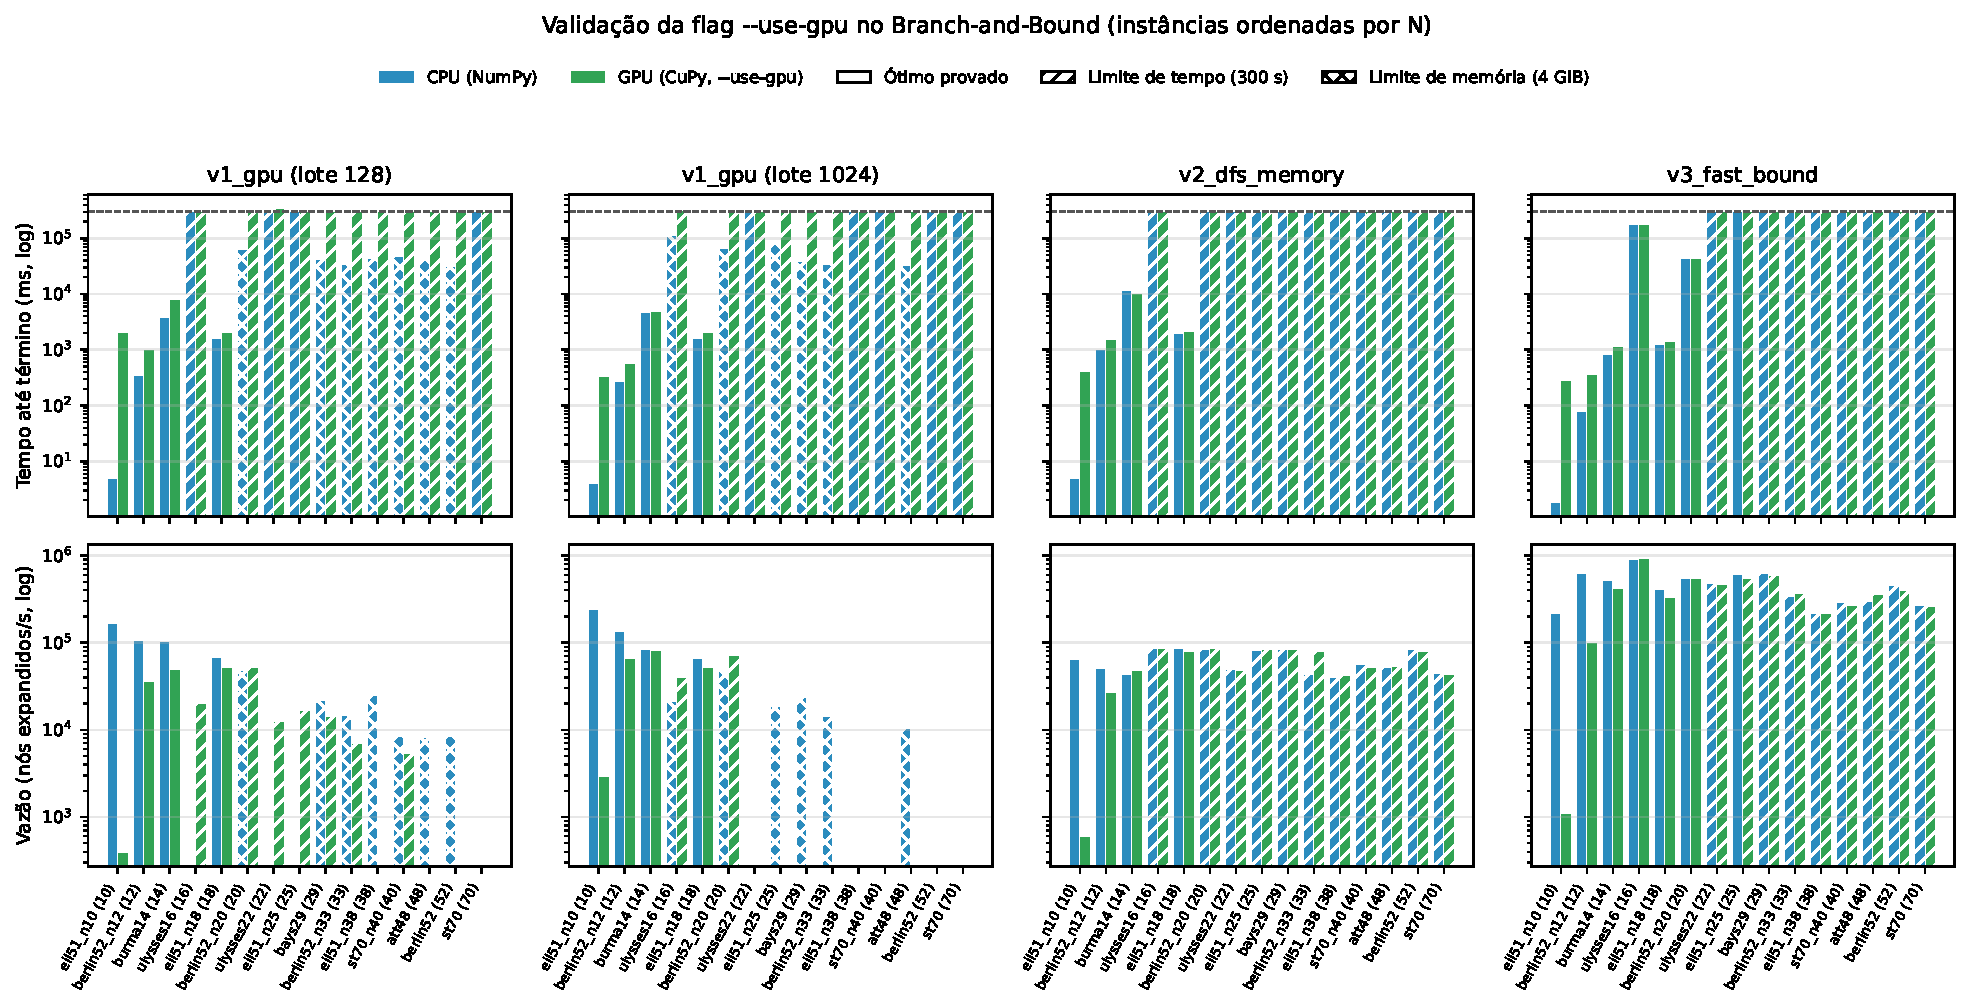
\includegraphics[width=\linewidth]{figures/fig6_gpu_validation.pdf}%
  }{\todoLab{Figura 6 ainda não gerada}}
  \caption{Bateria D. Tempo até o término (acima) e vazão em nós expandidos por segundo
  (abaixo), em CPU e GPU, para cada configuração. Instâncias ordenadas por $N$.}
  \label{fig:gpu}
\end{figure}

\section{Conclusões}
\label{sec:conclusoes}

Neste trabalho, analisamos diferentes algoritmos para o Problema do Caixeiro Viajante Euclidiano bidimensional (\texttt{EUC\_2D}), utilizando 15 instâncias da TSPLIB ($N \in [10, 70]$). Ao longo dos experimentos, foram realizadas otimizações graduais com base nas hipóteses levantadas e os resultados foram avaliados por meio de análises estatísticas de desempenho. A seguir, apresentamos as principais conclusões obtidas nas Baterias A--D.

\subsection{Algoritmos Aproximados: \textit{Twice-Around-The-Tree} e Christofides}
\label{sec:conc_aproximados}

Os resultados da Bateria~A (Seção~\ref{sec:res_aproximados}) mostram como a escolha das estruturas de dados pode influenciar o desempenho dos algoritmos polinomiais, além de permitir uma comparação prática entre os dois algoritmos aproximados:

\begin{itemize}
    \item \textbf{\textit{Twice-Around-The-Tree} (\texttt{v0} $\rightarrow$ \texttt{v1}):} a substituição do grafo completo dinâmico, do algoritmo de Kruskal $O(N^2 \log N)$ e do multigrafo duplicado $2T$ pelo Prim denso $\Theta(N^2)$ sobre uma matriz contígua e pelo percurso iterativo em pré-ordem $\Theta(N)$ reduziu consideravelmente o consumo de memória e o tempo de execução. Na instância \texttt{st70} ($N = 70$), por exemplo, o pico de memória passou de $655\text{ KiB}$ para $4{,}1\text{ KiB}$ ($\approx 160\times$), enquanto o tempo mediano caiu de $12{,}2\text{ ms}$ para $0{,}29\text{ ms}$ ($\approx 42\times$). Os resultados de memória ficaram próximos do comportamento teórico esperado, passando de $\Theta(N^2)$ na \texttt{v0} ($R^2 = 0{,}997$) para $\Theta(N)$ na \texttt{v1} ($R^2 = 0{,}996$).

    Em relação à qualidade das soluções, todas as 15 instâncias respeitaram a garantia de $2$-aproximação, com erro médio de $26{,}2\%$ e maior erro de $47{,}1\%$ em \texttt{eil51\_n38}. Mesmo assim, o algoritmo obteve soluções piores que as de Christofides em todas as instâncias e que as do Vizinho Mais Próximo em 12 das 15. Os erros foram maiores nas instâncias com alta entropia espacial ($\rho = 0{,}67$). Por outro lado, não foi encontrada uma relação relevante com o grau máximo da AGM ($\rho = 0{,}03$), contrariando essa expectativa da hipótese $H_{TA}$.

    \item \textbf{Christofides (\texttt{v0} $\rightarrow$ \texttt{v1}):} a remoção do grafo completo também trouxe melhorias para esse algoritmo. Na instância \texttt{st70}, o pico de memória caiu de $655\text{ KiB}$ para $341\text{ KiB}$ e o tempo total passou de $35{,}0\text{ ms}$ para $16{,}5\text{ ms}$. Como previsto na hipótese $H_C$, os ganhos foram limitados pelo emparelhamento perfeito mínimo (Blossom), responsável por $91{,}5\%$ do tempo de execução e por todo o pico de memória da \texttt{v1}.

    Os experimentos também mostraram que o custo do algoritmo está mais relacionado à quantidade de vértices de grau ímpar $|I|$ da AGM do que ao número total de vértices $N$. O ajuste cúbico em $|I|^3$ obteve $R^2 = 0{,}875$, contra $0{,}663$ para $N^3$, enquanto o ajuste de memória em $|I|^2$ atingiu $R^2 = 0{,}999$. Quanto à qualidade das soluções, Christofides apresentou erro médio de $7{,}4\%$ e máximo de $15{,}5\%$, bem abaixo dos $50\%$ previstos pela garantia teórica. Além disso, os resultados se mantiveram relativamente estáveis diante das diferentes características geométricas e estruturais das instâncias ($|\rho| < 0{,}47$).

    \item \textbf{Influência do tamanho das instâncias nas regressões de tempo:} para $N \le 70$, algumas subrotinas otimizadas, como Prim denso, pré-ordem, Hierholzer e Varredura de Graham, executam em menos de $1\text{ ms}$. Nesses casos, o custo fixo do interpretador e as variações causadas pelo escalonador dificultam a observação do crescimento assintótico, o que ajuda a explicar os baixos valores de $R^2$ nas regressões de tempo. Já os resultados de memória ficaram muito próximos das complexidades teóricas ($R^2 \ge 0{,}996$).
\end{itemize}

\subsection{Estratégias de Inicialização (\textit{Warm-Start})}
\label{sec:conc_warmstarts}

Na Bateria~C (Seção~\ref{sec:res_warmstart}), verificamos que as cinco estratégias de inicialização tiveram um custo de execução muito baixo em comparação com a busca exata. Christofides levou, no máximo, $29\text{ ms}$, enquanto a Inserção em Fecho Convexo levou até $4\text{ ms}$. Já a busca exata chegou a durar 30 minutos. Dessa forma, mais importante do que o tempo gasto na inicialização foi a qualidade da solução encontrada, ou seja, o quanto o limite superior inicial $UB_0$ estava próximo do ótimo antes de iniciar a DFS.

\begin{itemize}
    \item \textbf{Inserção em Fecho Convexo}: a otimização com validação preguiçosa reduziu a complexidade para $O(N^2 \log N)$, com um ajuste temporal de $R^2 = 0{,}714$. Além de apresentar um baixo tempo de execução, essa estratégia encontrou as melhores soluções iniciais em 14 das 15 instâncias, com erro médio de apenas $2{,}2\%$, alcançando o ótimo em quatro delas. Também observamos que, quanto maior a proporção de pontos no fecho convexo, menor tende a ser o erro ($\rho = -0{,}70$). Quando utilizada como \textit{warm-start}, a estratégia reduziu em média $41{,}5\%$ dos nós expandidos nas instâncias resolvidas. Em \texttt{eil51\_n25}, por exemplo, o número de nós expandidos passou de 206 milhões para 14 milhões, enquanto o tempo de execução caiu de $341\text{ s}$ para $26{,}1\text{ s}$.

    \item \textbf{Christofides}: entre os algoritmos com garantia formal de aproximação analisados, foi o que encontrou as melhores soluções iniciais, respeitando a garantia de $1{,}5 \cdot OPT$. Os erros variaram entre $1{,}2\%$ e $15{,}5\%$, com média de $7{,}4\%$. Na instância \texttt{ulysses16}, chegou a superar a Inserção em Fecho Convexo, com erro de $1{,}2\%$ contra $1{,}5\%$. Como estratégia de inicialização, reduziu em média $3{,}4\%$ dos nós expandidos e, em \texttt{eil51\_n25}, diminuiu o tempo de execução de $341\text{ s}$ para $295\text{ s}$. Essa redução foi menor porque a DFS geralmente encontra boas soluções logo no início da busca, superando as rotas fornecidas por Christofides. Por outro lado, o algoritmo se mostrou útil nas instâncias que atingiram o limite de 30 minutos (\texttt{TL}). Em comparação com a inicialização fria, os erros finais passaram de $4{,}5\%$ para $2{,}9\%$ em \texttt{ulysses22}, de $9{,}1\%$ para $6{,}8\%$ em \texttt{bays29} e de $18{,}6\%$ para $9{,}1\%$ em \texttt{st70}.

    \item \textbf{Vizinho Mais Próximo}: apesar do baixo tempo de execução e da complexidade $\Theta(N^2)$, a escolha gulosa dos vértices resultou em soluções com erro médio de $16{,}4\%$. Os erros variaram de $5{,}1\%$ em \texttt{eil51\_n38} a $41{,}6\%$ em \texttt{ulysses16}, com tendência a resultados piores em instâncias mais alongadas ($\rho = 0{,}48$ para a razão de aspecto). Na Bateria~C, a redução média dos nós expandidos foi de apenas $0{,}1\%$, pois a estratégia \textit{Best-Child-First} da \texttt{v3} geralmente consegue encontrar soluções melhores logo no início da DFS. Ainda assim, em algumas instâncias, a inicialização trouxe benefícios. Em \texttt{eil51\_n38}, por exemplo, o erro ao atingir o limite de tempo foi de $2{,}7\%$, contra $7{,}2\%$ da inicialização fria.

    \item \textbf{\textit{Twice-Around-The-Tree}}: mesmo com tempo de execução inferior a um milissegundo na \texttt{v1} e garantia teórica de $2 \cdot OPT$, o algoritmo apresentou erros entre $7{,}8\%$ e $47{,}1\%$, com média de $26{,}2\%$. Na prática, as soluções iniciais foram piores do que aquelas encontradas pela DFS logo no início da busca. Por isso, a redução média dos nós expandidos foi de $0{,}0\%$, e a estratégia não trouxe melhorias nas instâncias que atingiram o limite de tempo. Os erros finais foram os mesmos da inicialização fria, como os $18{,}6\%$ em \texttt{st70} e os $9{,}1\%$ em \texttt{bays29}.

    \item \textbf{Inicialização Fria (\textit{Cold Start})}: foi utilizada como base de comparação para as demais estratégias, com complexidade $\Theta(N)$ e sem considerar a distribuição espacial dos vértices. Graças à ordenação dos filhos na \texttt{v3}, seus tempos de execução nas instâncias menores foram próximos aos do Vizinho Mais Próximo e do \textit{Twice-Around-The-Tree}. No entanto, essa abordagem não fornece um limite inicial que favoreça as podas e pode resultar em soluções de menor qualidade quando a execução é interrompida pelo limite de tempo.
\end{itemize}


\subsection{Busca Exata (\textit{Branch-and-Bound} \texttt{v0}--\texttt{v3}) e Aceleração em GPU}
\label{sec:conc_bnb_gpu}

As otimizações realizadas na Bateria~B (Seção~\ref{sec:res_bnb}) e a comparação entre CPU e GPU na Bateria~D (Seção~\ref{sec:res_gpu}) permitiram identificar os principais problemas de desempenho da busca exata implementada em Python.

\begin{itemize}
    \item \textbf{\texttt{v0\_naive} versus \texttt{v1\_gpu} (velocidade e consumo de memória):} na \texttt{v0}, o recálculo de complexidade $O(N^2)$ para cada candidato limitou o processamento a aproximadamente $1\,000\text{ nós/s}$. Com isso, a versão atingiu o limite de tempo de 120~s antes de esgotar a memória disponível, chegando a um pico de $948\text{ MB}$. A vetorização em lotes da \texttt{v1} aumentou a taxa de processamento em $23\times$, chegando a aproximadamente $24\,000\text{ nós/s}$. Em \texttt{burma14}, por exemplo, o tempo caiu de $64{,}3\text{ s}$ para $4{,}37\text{ s}$.

    Apesar desse ganho, o processamento mais rápido fez com que a fila da busca \textit{Best-First} crescesse exponencialmente, chegando à ordem de $10^7$ estados. Como resultado, o limite de 4~GiB de memória foi atingido (\texttt{OOM}) em todas as 11 instâncias maiores, entre $28\text{ s}$ e $69\text{ s}$ de execução.

    \item \textbf{\texttt{v2\_dfs\_memory} versus \texttt{v3\_fast\_bound} (memória e taxa de processamento):} a utilização de DFS \textit{in-place} na \texttt{v2} resolveu o problema de estouro de memória, mantendo a pilha com no máximo $N$ elementos e o consumo do processo estável em $196\text{ MB}$. Entretanto, as alocações de vetores a cada nó ainda limitavam o processamento a cerca de $50\,000\text{ nós/s}$, e a DFS expandia mais estados que a busca \textit{Best-First}.

    A \texttt{v3} reduziu o custo de processamento de cada nó ao combinar o cálculo incremental escalar do limite em $\Theta(1)$, o uso de \textit{bitmask} inteiro e a quebra de simetria. Essas mudanças aumentaram a taxa de processamento em $8\times$ em relação à \texttt{v2}, chegando a aproximadamente $420\,000\text{ nós/s}$. Embora a quebra de simetria possa atrasar a descoberta de boas soluções em algumas instâncias, como \texttt{eil51\_n18}, a \texttt{v3} foi a versão mais rápida em todos os casos resolvidos. Ela também foi a única a resolver \texttt{berlin52\_n20} dentro de 120~s e conseguiu provar a otimalidade em 7 das 15 instâncias dentro do limite de 30 minutos.

    \item \textbf{Uso da GPU:} a opção \texttt{--use-gpu} não trouxe ganhos de velocidade para nenhuma das versões testadas na Bateria~D. A razão mediana entre as taxas de processamento da GPU e da CPU ficou entre $0{,}89$ e $0{,}99$. Além disso, o custo de inicialização do CUDA prejudicou o desempenho nas instâncias menores, como \texttt{eil51\_n10}, que levou $2{,}1\text{ s}$ com GPU e apenas $4\text{ ms}$ com CPU. Para as instâncias analisadas ($N \le 70$), os lotes de processamento não foram grandes o suficiente para aproveitar toda a capacidade da GPU, e o principal gargalo continuou sendo a manipulação da árvore de busca e da fila na CPU. Esse resultado também reforça a decisão de manter o \textit{Twice-Around-The-Tree} executando exclusivamente na CPU.
\end{itemize}

\subsection{Sensibilidade Topológica e Recomendações Finais}
\label{sec:conc_sintese}

A análise de sensibilidade (Seção~\ref{sec:res_sensibilidade}) mostrou que a distribuição espacial dos vértices pode influenciar o desempenho da busca exata mais do que a quantidade de vértices da instância. Distribuições com aglomerados e pontos isolados, caracterizadas por um alto coeficiente de variação das distâncias ao vizinho mais próximo e das arestas da AGM ($\rho = 0{,}90$), além de baixa entropia espacial ($\rho = -0{,}81$), fazem com que o limite inferior de grau~2 na raiz fique mais distante do ótimo. Em \texttt{ulysses22}, por exemplo, a razão $LB_0/OPT$ foi de $0{,}639$, enquanto em \texttt{eil51\_n38} foi de $0{,}936$.

Essa diferença ajuda a explicar por que algumas instâncias menores exigiram mais esforço computacional que outras maiores. A instância \texttt{ulysses16} ($N = 16$) exigiu $340\times$ mais nós e levou $325\text{ s}$, enquanto \texttt{eil51\_n18} ($N = 18$) levou apenas $1{,}6\text{ s}$. De forma semelhante, \texttt{ulysses22} ($N = 22$) ultrapassou o limite de 30 minutos, enquanto \texttt{eil51\_n25} ($N = 25$) foi resolvida em $26{,}1\text{ s}$ utilizando a Inserção em Fecho Convexo.

Com base nos resultados, para instâncias euclidianas pequenas ou com distribuição espacial mais regular ($N \le 25$), a versão \texttt{v3} do \textit{Branch-and-Bound}, inicializada com a Inserção em Fecho Convexo, mostrou-se uma boa escolha por combinar a possibilidade de provar a otimalidade, consumo de memória $\Theta(N)$ e melhor tempo total. Para instâncias maiores ou com muitos aglomerados, a Inserção em Fecho Convexo oferece soluções de boa qualidade em poucos milissegundos, enquanto Christofides é uma alternativa indicada quando é necessário garantir uma aproximação de pior caso de $1{,}5\cdot OPT$.



\bibliographystyle{sbc}
\bibliography{references}

\end{document}
